\documentclass[a4paper,10pt,titlepage,leqno]{article}

% ── Encodage & langue ──
\usepackage[french]{babel}
\usepackage[T1]{fontenc}
\usepackage[utf8]{inputenc}

% ── Mise en page ──
\usepackage[margin=2.4cm, top=2.8cm, bottom=2.8cm]{geometry}
\usepackage{parskip}
\setlength{\parskip}{0.45em}

% ── Mathématiques ──
\usepackage{amsmath,amssymb,amsthm}
\newtheorem{proposition}{Proposition}
\newtheorem{definition}{Définition}

% ── Tableaux & figures ──
\usepackage{booktabs}
\usepackage{graphicx}
\usepackage{float}
\usepackage{subcaption}
\usepackage{multirow}
\usepackage{array}

% ── Couleurs & encadrés ──
\usepackage[dvipsnames,table]{xcolor}
\usepackage[most]{tcolorbox}

\definecolor{navydark}{HTML}{1B2A4A}
\definecolor{navymid}{HTML}{2B4C7E}
\definecolor{navylight}{HTML}{E8EEF4}
\definecolor{navypale}{HTML}{F0F4F8}
\definecolor{navyaccent}{HTML}{3D6098}

\newtcolorbox{theorybox}[1][]{
  colback=navylight, colframe=navydark,
  fonttitle=\bfseries\color{white}, title={#1},
  boxrule=0.8pt, arc=3pt, left=6pt, right=6pt, top=4pt, bottom=4pt,
  coltitle=white, colbacktitle=navydark
}

\newtcolorbox{resultbox}[1][]{
  colback=navypale, colframe=navyaccent,
  fonttitle=\bfseries\color{white}, title={#1},
  boxrule=0.8pt, arc=3pt, left=6pt, right=6pt, top=4pt, bottom=4pt,
  coltitle=white, colbacktitle=navyaccent
}

% ── Divers ──
\usepackage{hyperref}
\hypersetup{colorlinks=true, linkcolor=navydark, citecolor=navydark, urlcolor=navymid}
\usepackage{tikz}
\usetikzlibrary{positioning,shapes.geometric,arrows.meta}
\usepackage{enumitem}
\setlist{nosep, leftmargin=1.4em}
\usepackage{titlesec}
\titleformat{\section}{\Large\bfseries\color{navydark}}{\thesection}{0.7em}{}
\titleformat{\subsection}{\large\bfseries\color{navymid}}{\thesubsection}{0.6em}{}
\titleformat{\subsubsection}{\normalsize\bfseries\color{navyaccent}}{\thesubsubsection}{0.5em}{}

% ── En-tête & pied de page (page de garde) ──
\usepackage{fancyhdr}
\pagestyle{fancy}
\fancyhf{}
\rhead{Octobre 2025}
\chead{5OD21 Optimisation Discrète}
\lhead{Selim-Antoine Lali, Gabriel Bus}
\cfoot{Page \thepage}

% ══════════════════════════════════════════════════════════════════════════
\title{\vspace{-1cm}\textbf{Arbres de décision optimaux par programmation linéaire en nombres entiers}\\[0.3em]
\large Égalités valides, équité, features dérivées et formulation binaire}
\author{Gabriel Bus\\[0.5em]\normalsize Projet d'optimisation en nombres entiers -- ENSTA Paris}
\date{Mars 2026}

\begin{document}
\makeatletter
\begin{titlepage}
  \null\vfill
  \begin{center}
    % Logo ENSTA Paris -- placer le fichier logo.png dans doc/
    \includegraphics[width=0.35\textwidth]{logo.png}\\[2cm]
    \LARGE\bfseries\@title\par
    \vspace{1.5cm}
    \large\@author\par
    \vspace{0.8cm}
    \normalsize\@date\par
  \end{center}
  \vfill\null
\end{titlepage}
\makeatother
\thispagestyle{empty}
\newpage
\setcounter{page}{1}

% ── Abstract ──
\begin{abstract}
Ce rapport présente quatre extensions d'un modèle MIP pour la construction d'arbres de décision optimaux.
La \textbf{Partie~1} exploite les égalités valides (linked sets et opposite box corners) pour renforcer la relaxation linéaire et accélérer le branch-and-bound.
La \textbf{Partie~2} intègre des contraintes d'équité (parité démographique, equal opportunity) et étudie le compromis équité--précision.
La \textbf{Partie~3} propose un algorithme de génération de features dérivées (ratios, différences, produits) sélectionnées par gain de Gini.
La \textbf{Partie~4} implémente la formulation univariée pour jeux de données binaires, son renforcement par Equivalent Sets et des bornes alternatives sur les variables~$\theta$.
Les expériences sont menées sur cinq jeux de données~: \texttt{iris}, \texttt{seeds}, \texttt{wine} (fournis), \texttt{glass} et \texttt{ecoli} (UCI), avec des profondeurs $D\in\{2,3\}$.
Les limites de temps CPLEX sont centralisées dans \texttt{src/datasets\_config.jl} (\texttt{IOML\_TL\_MAIN}, \texttt{IOML\_TL\_PARTS}) ; les tableaux numériques correspondent aux fichiers CSV du dossier \texttt{results/} au moment de la rédaction.
Des figures complémentaires (réduction B\&B, compromis équité) sont générées par \texttt{scripts/generate\_all\_plots.jl} en plus des graphiques de base.
\end{abstract}

\tableofcontents
\vspace{0.8em}

% ══════════════════════════════════════════════════════════════════════════
\section{Partie 1 -- Égalités valides et cutting planes}
\label{sec:part1}
% ══════════════════════════════════════════════════════════════════════════

\subsection{Méthode}

On travaille en arbres univariés avec un modèle à \emph{flux unitaire} : chaque échantillon~$i$ envoie exactement une unité de flot vers une feuille ($\sum_{t \in \mathcal{L}} u^i_{t,w} = 1$). L'objectif est de maximiser le nombre de bien classés. Pour renforcer la relaxation linéaire, on ajoute des \textbf{égalités valides} détectées automatiquement sur les données d'entraînement, puis on résout le MIP.

Deux familles d'égalités sont exploitées :

\begin{enumerate}
  \item \textbf{Linked sets} (Section~4 du cours) : triplets $(P, Q, \bar{j})$ tels que $|P|=|Q|$ et les points de $P$ et $Q$ coïncident sur toutes les features sauf $\bar{j}$, avec un cycle sur $\bar{j}$.
  \item \textbf{Opposite box corners} : paires de coins opposés d'une boîte $B(p^-, p^+)$ dans l'espace des features.
\end{enumerate}

Un algorithme de \textbf{cutting plane} résout d'abord la relaxation LP, ajoute uniquement les égalités violées, et répète jusqu'à convergence avant de résoudre le MIP complet. Un mécanisme d'\textbf{arrondi} des features à $k$ décimales augmente le nombre d'égalités détectables.

\subsection{Questions théoriques}

\begin{theorybox}[Définition et proposition : linked sets]

\begin{definition}[Linked set]
Soit $\mathcal{J}$ l'ensemble des features et $\mathcal{I}$ l'ensemble des échantillons. Un \textbf{linked set} est un triplet $(P, Q, \bar{j})$ où $\bar{j} \in \mathcal{J}$ est une feature distinguée et $P = \{p_1, \ldots, p_{n_s}\}$, $Q = \{q_1, \ldots, q_{n_s}\}$ sont deux sous-ensembles de $\mathcal{I}$ de même cardinal $n_s$ vérifiant~:
\begin{enumerate}[label=(\roman*)]
  \item \textbf{Coïncidence hors $\bar{j}$} : $x_{p_k, j} = x_{q_k, j}$ pour tout $k \in \{1, \ldots, n_s\}$ et tout $j \in \mathcal{J} \setminus \{\bar{j}\}$.
  \item \textbf{Cycle sur $\bar{j}$} : $x_{q_k, \bar{j}} = x_{p_{k+1}, \bar{j}}$ pour tout $k \in \{1, \ldots, n_s\}$, avec la convention circulaire $p_{n_s+1} \triangleq p_1$.
\end{enumerate}
La condition~(i) signifie que $p_k$ et $q_k$ sont ``jumeaux'' sur toutes les features sauf $\bar{j}$. La condition~(ii) chaîne les valeurs de $\bar{j}$ en un cycle~: la valeur de $q_k$ sur $\bar{j}$ est celle de $p_{k+1}$, et celle de $q_{n_s}$ boucle sur $p_1$.
\end{definition}

\begin{proposition}
Pour chaque linked set $(P, Q, \bar{j})$, l'égalité suivante est valide pour toute solution réalisable du modèle à flux unitaire~:
\begin{equation}
  \sum_{\ell \in \mathcal{L}} \sum_{k=1}^{n_s} \bigl( u_{\ell,w}^{p_k} - u_{\ell,w}^{q_k} \bigr) = 0.
  \label{eq:linked}
\end{equation}
\end{proposition}

\begin{proof}
Dans le modèle à flux unitaire, chaque échantillon~$i$ envoie exactement une unité de flot vers une unique feuille~:
\[
  \forall\, i \in \mathcal{I}, \qquad \sum_{\ell \in \mathcal{L}} u_{\ell,w}^{i} = 1.
\]
Considérons un indice $k \in \{1, \ldots, n_s\}$ quelconque. En appliquant cette contrainte successivement à $p_k$ et $q_k$, on obtient~:
\[
  \sum_{\ell \in \mathcal{L}} u_{\ell,w}^{p_k} = 1 \qquad \text{et} \qquad \sum_{\ell \in \mathcal{L}} u_{\ell,w}^{q_k} = 1,
\]
d'où $\sum_{\ell \in \mathcal{L}} \bigl( u_{\ell,w}^{p_k} - u_{\ell,w}^{q_k} \bigr) = 1 - 1 = 0$.

Ce résultat est valable pour \emph{chaque} $k$ individuellement, indépendamment de la structure de linked set. En sommant sur $k = 1, \ldots, n_s$~:
\[
  \sum_{\ell \in \mathcal{L}} \sum_{k=1}^{n_s} \bigl( u_{\ell,w}^{p_k} - u_{\ell,w}^{q_k} \bigr) = \sum_{k=1}^{n_s} 0 = 0.
\]

\textbf{Remarque.} La structure de linked set (conditions (i) et (ii)) n'est pas nécessaire pour la validité de l'égalité~\eqref{eq:linked} au niveau entier --- la contrainte de flux unitaire suffit. Cependant, la structure de linked set garantit que cette égalité est \emph{utile} au niveau de la relaxation LP~: les conditions de coïncidence et de cycle font que les solutions fractionnaires du LP peuvent violer~\eqref{eq:linked}, ce qui en fait un plan coupant efficace. \qedhere
\end{proof}
\end{theorybox}

\begin{theorybox}[Définition et proposition : opposite box corners]

\begin{definition}[Boîte et coins opposés]
Une \textbf{boîte} $B(p^-, p^+) \subset \mathbb{R}^{|\mathcal{J}|}$ est définie par deux vecteurs $p^-, p^+ \in \mathbb{R}^{|\mathcal{J}|}$ avec $p^-_j \leq p^+_j$ pour tout $j$~:
\[
  B(p^-, p^+) = \bigl\{ v \in \mathbb{R}^{|\mathcal{J}|} \;\big|\; p^-_j \leq v_j \leq p^+_j, \;\forall\, j \in \mathcal{J} \bigr\}.
\]
Deux points $i_a, i_b$ de cette boîte sont des \textbf{coins opposés} si, pour chaque dimension $j$, l'un vaut $p^-_j$ et l'autre $p^+_j$~: $\{x_{i_a, j}, x_{i_b, j}\} = \{p^-_j, p^+_j\}$ pour tout $j \in \mathcal{J}$.
\end{definition}

\begin{proposition}
Sous flux unitaire, pour deux paires distinctes de coins opposés $(i_1,i_2)$ et $(i_3,i_4)$ d'une même boîte $B(p^-, p^+)$, l'égalité
\[
u^{i_1}_{r,\ell(r)} + u^{i_2}_{r,\ell(r)} = u^{i_3}_{r,\ell(r)} + u^{i_4}_{r,\ell(r)}
\]
est valide dans le modèle univarié, où $r$ désigne la racine et $\ell(r) = 2r$ son fils gauche.
\end{proposition}

\begin{proof}
Dans le modèle univarié, la racine $r$ branche sur une unique feature $\bar{j} \in \mathcal{J}$ avec un seuil $b_r$. Un point $i$ est envoyé vers le fils gauche $\ell(r)$ (i.e.\ $u^i_{r,\ell(r)} = 1$) si et seulement si $x_{i,\bar{j}} + \mu^- \leq b_r$, où $\mu^- = \min_j \mu_j$ est la constante de marge du modèle. Sinon, $u^i_{r,\ell(r)} = 0$ (le point va à droite).

Puisque $i_1, i_2, i_3, i_4$ sont des coins de la boîte $B(p^-, p^+)$, leurs coordonnées sur $\bar{j}$ ne prennent que deux valeurs~: $p^-_{\bar{j}}$ et $p^+_{\bar{j}}$ (avec $p^-_{\bar{j}} \leq p^+_{\bar{j}}$). On distingue trois cas selon la position du seuil~:

\begin{enumerate}[leftmargin=2em]
  \item \textbf{Cas $b_r < p^-_{\bar{j}} + \mu^-$.} Aucun point ne satisfait $x_{i,\bar{j}} + \mu^- \leq b_r$, car $x_{i,\bar{j}} \geq p^-_{\bar{j}}$ pour tout coin. Donc $u^i_{r,\ell(r)} = 0$ pour $i \in \{i_1, i_2, i_3, i_4\}$, et les deux membres valent $0 + 0 = 0$.

  \item \textbf{Cas $p^-_{\bar{j}} + \mu^- \leq b_r \leq p^+_{\bar{j}} + \mu^-$.} Le seuil sépare les deux valeurs~: les points avec $x_{i,\bar{j}} = p^-_{\bar{j}}$ vont à gauche ($u = 1$) et ceux avec $x_{i,\bar{j}} = p^+_{\bar{j}}$ vont à droite ($u = 0$). Or, dans chaque paire de coins opposés, par définition, exactement un point a $x_{i,\bar{j}} = p^-_{\bar{j}}$ et l'autre a $x_{i,\bar{j}} = p^+_{\bar{j}}$. Donc chaque membre vaut $1 + 0 = 1$.

  \item \textbf{Cas $b_r > p^+_{\bar{j}} + \mu^-$.} Tous les points satisfont $x_{i,\bar{j}} + \mu^- \leq b_r$, donc $u^i_{r,\ell(r)} = 1$ pour tout~$i$. Les deux membres valent $1 + 1 = 2$.
\end{enumerate}

Dans les trois cas, le membre gauche est égal au membre droit. L'égalité est donc valide pour toute solution entière réalisable du modèle univarié avec flux unitaire.

\textbf{Remarque.} Comme pour les linked sets, l'intérêt de cette égalité réside dans son effet sur la relaxation LP~: les coins opposés d'une même boîte ont des positions symétriques par rapport au seuil de branchement, ce qui force la relaxation fractionnaire à respecter cette symétrie. Plus il y a de paires de coins opposés dans les données (favorisé par l'arrondi), plus le polytope de la relaxation est resserré. \qedhere
\end{proof}
\end{theorybox}

\begin{figure}[H]
\centering
\begin{tikzpicture}[scale=1.1]
  \draw[thick, fill=gray!5] (0,0) rectangle (4,3);
  \node at (2,1.5) {\small $B(p^-, p^+)$};
  \fill[navydark] (0,0) circle (3pt) node[below left] {\small $i_1$};
  \fill[navydark] (4,3) circle (3pt) node[above right] {\small $i_2$};
  \draw[navydark, thick, dashed] (0,0) -- (4,3);
  \fill[navyaccent] (0,3) circle (3pt) node[above left] {\small $i_3$};
  \fill[navyaccent] (4,0) circle (3pt) node[below right] {\small $i_4$};
  \draw[navyaccent, thick, dashed] (0,3) -- (4,0);
\end{tikzpicture}
\caption{Boîte 2D avec deux paires de coins opposés $(i_1,i_2)$ en bleu foncé et $(i_3,i_4)$ en bleu clair.}
\label{fig:box}
\end{figure}

\subsection{Résultats expérimentaux}

\paragraph{Protocole.} Cinq jeux de données~: \texttt{iris} (4~features, 120/30 train/test), \texttt{seeds} (6~features, 168/42), \texttt{wine} (13~features, 142/36), \texttt{glass} (9~features, classification de types de verre), \texttt{ecoli} (7~features, localisation de protéines). Données normalisées dans $[0,1]$. Profondeurs $D \in \{2,3\}$. Limite CPLEX pour \texttt{run\_part1}~: \texttt{DEFAULT\_TIME\_LIMIT\_PARTS} (défaut 300\,s, surcharge \texttt{IOML\_TL\_PARTS}) ; les valeurs du tableau~\ref{tab:part1} proviennent de \texttt{part1\_results.csv} (run récent avec limite 300\,s). On compare la résolution \emph{sans} et \emph{avec} égalités (linked sets + opposite box corners), avec différents niveaux d'arrondi (aucun, 1, 2 décimales).

\begin{table}[H]
\centering
\caption{Résultats sans arrondi, $D=2$ : temps, nœuds B\&B et erreurs (source : \texttt{part1\_results.csv}, run 300\,s).}
\label{tab:part1}
\small
\begin{tabular}{@{}l cc cc cc@{}}
\toprule
 & \multicolumn{2}{c}{\textbf{Temps (s)}} & \multicolumn{2}{c}{\textbf{Nœuds B\&B}} & \multicolumn{2}{c}{\textbf{Err.\ test}} \\
\cmidrule(lr){2-3}\cmidrule(lr){4-5}\cmidrule(lr){6-7}
Dataset & Sans & Avec & Sans & Avec & Sans & Avec \\
\midrule
iris   & 1{,}3  & 0{,}9  & 1181   & 1070   & 1 & 1 \\
seeds  & 11{,}6 & 11{,}6 & 30808  & 30808  & 2 & 2 \\
wine   & 12{,}1 & 12{,}2 & 23283  & 23283  & 2 & 2 \\
glass  & 263{,}6 & 264{,}4 & 843168 & 818825 & 17 & 17 \\
ecoli  & 3{,}1  & 3{,}0  & 2160   & 2160   & 6 & 6 \\
\bottomrule
\end{tabular}
\end{table}

\begin{figure}[H]
\centering
\begin{subfigure}[t]{0.48\textwidth}
  \centering
  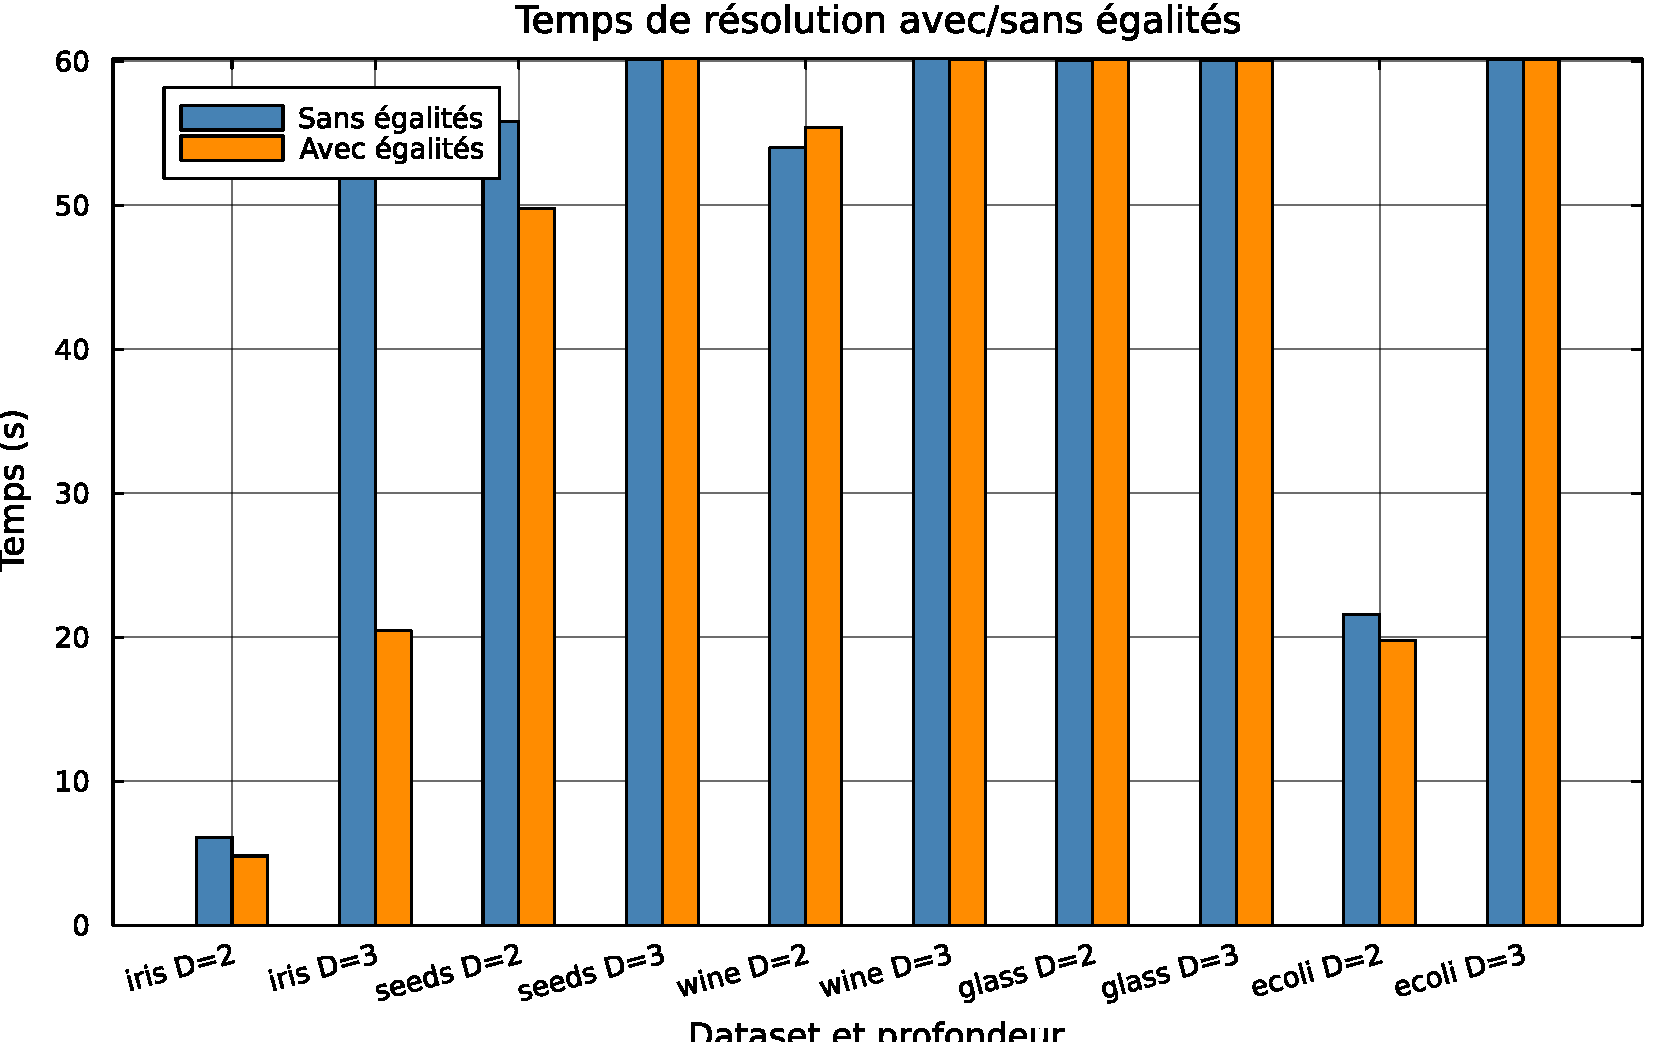
\includegraphics[width=\textwidth]{figures/part1_time_comparison.pdf}
  \caption{Temps de résolution.}
\end{subfigure}
\hfill
\begin{subfigure}[t]{0.48\textwidth}
  \centering
  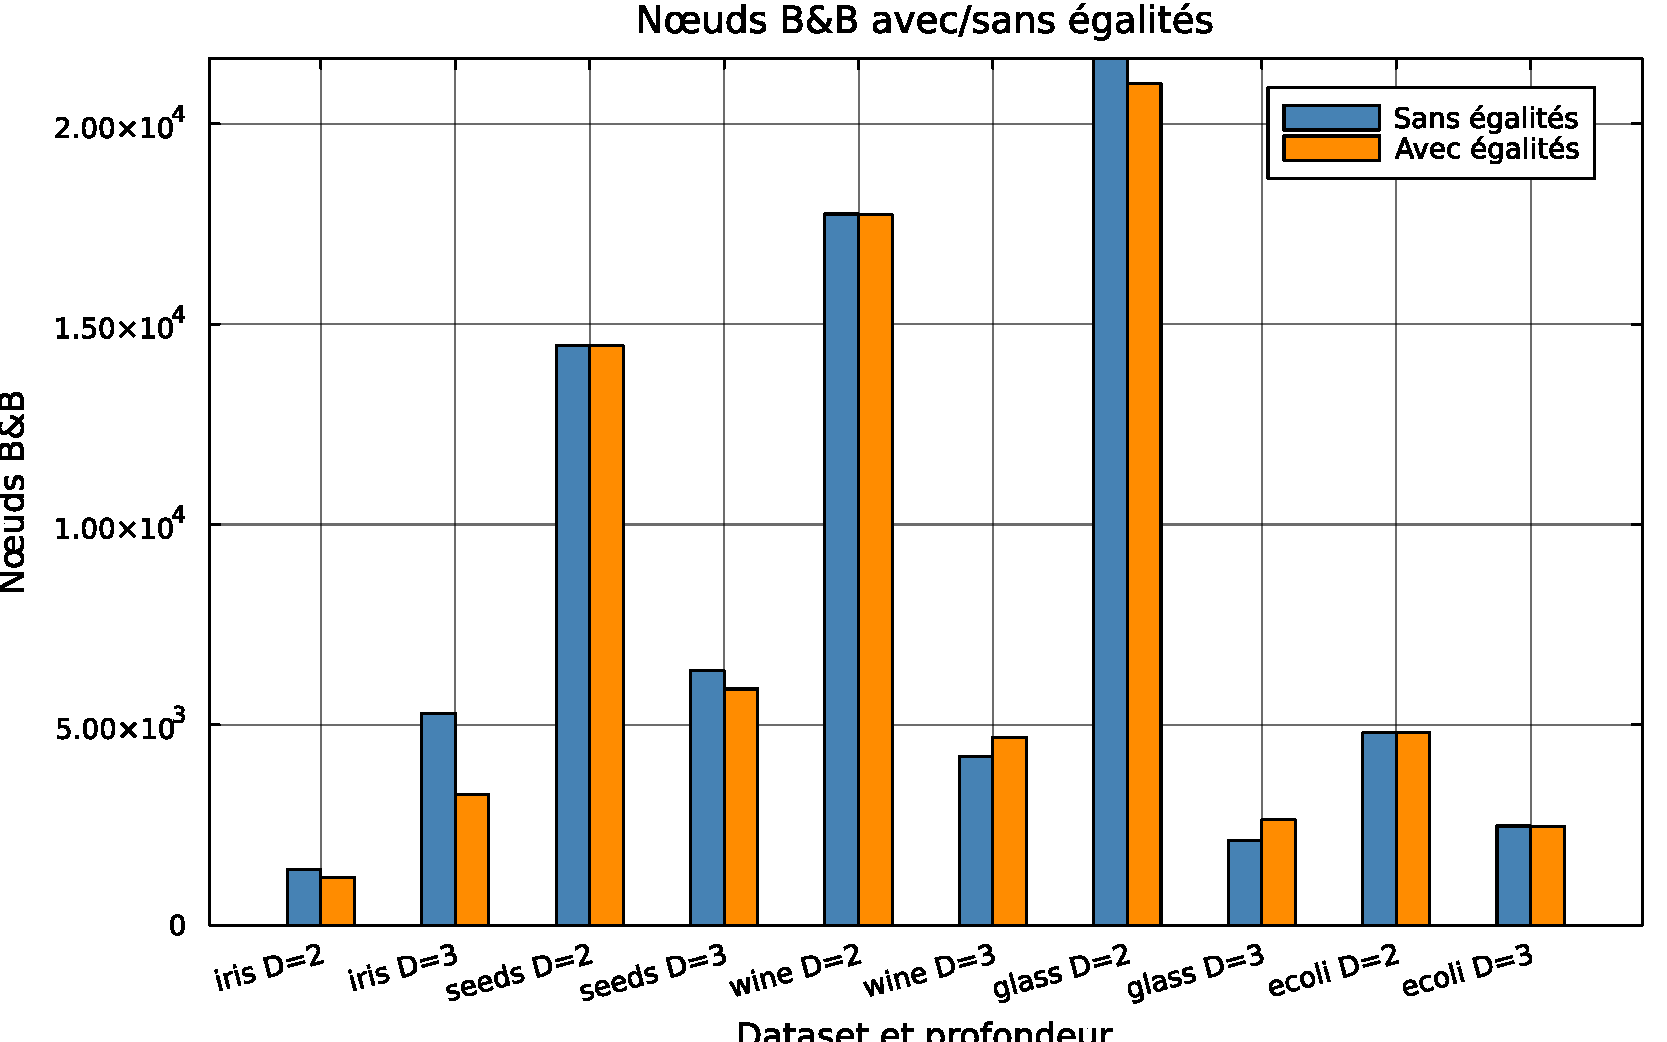
\includegraphics[width=\textwidth]{figures/part1_nodes_comparison.pdf}
  \caption{Nœuds de branch-and-bound.}
\end{subfigure}
\caption{Comparaison avec/sans égalités (sans arrondi) pour chaque dataset et profondeur.}
\label{fig:part1_comparison}
\end{figure}

\begin{figure}[H]
\centering
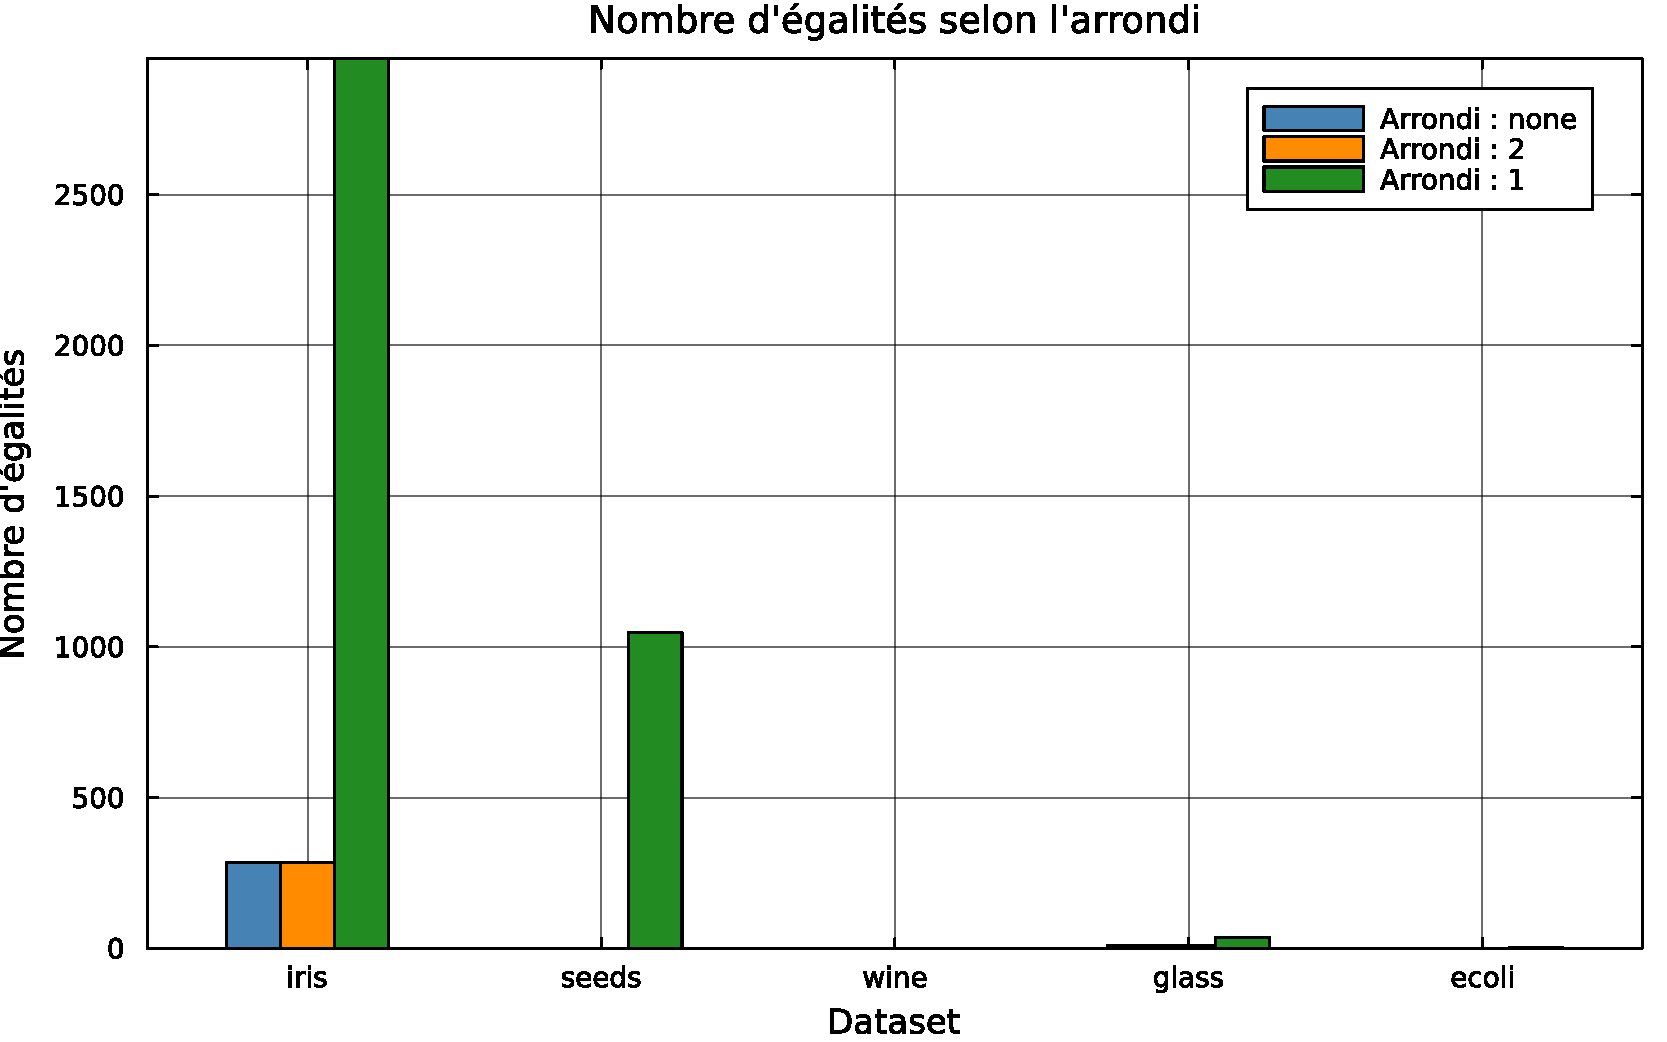
\includegraphics[width=0.65\textwidth]{figures/part1_equalities_by_rounding.pdf}
\caption{Nombre d'égalités détectées selon le niveau d'arrondi ($D=2$, config avec égalités).}
\label{fig:part1_rounding}
\end{figure}

\begin{figure}[H]
\centering
\begin{subfigure}[t]{0.48\textwidth}
  \centering
  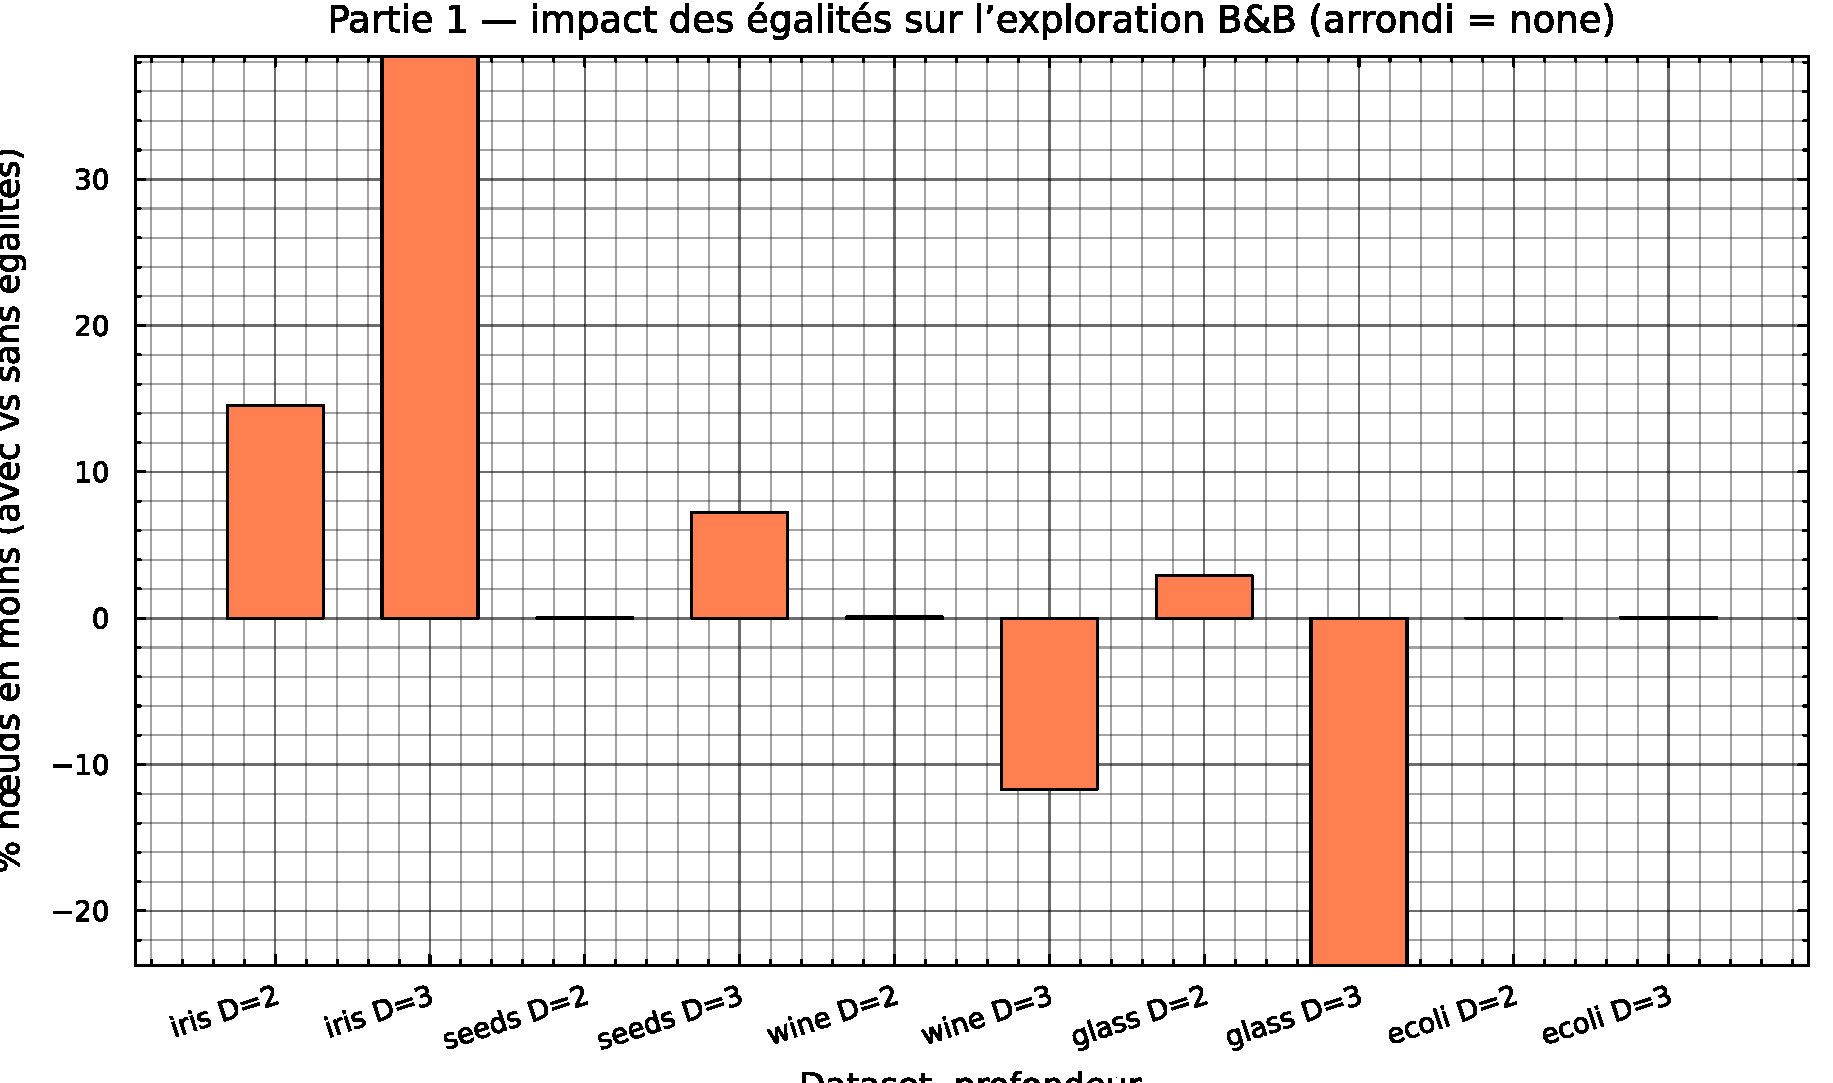
\includegraphics[width=\textwidth]{figures/part1_bb_node_reduction_pct.pdf}
  \caption{Réduction relative des nœuds B\&B (avec vs sans égalités, arrondi \texttt{none}).}
\end{subfigure}
\hfill
\begin{subfigure}[t]{0.48\textwidth}
  \centering
  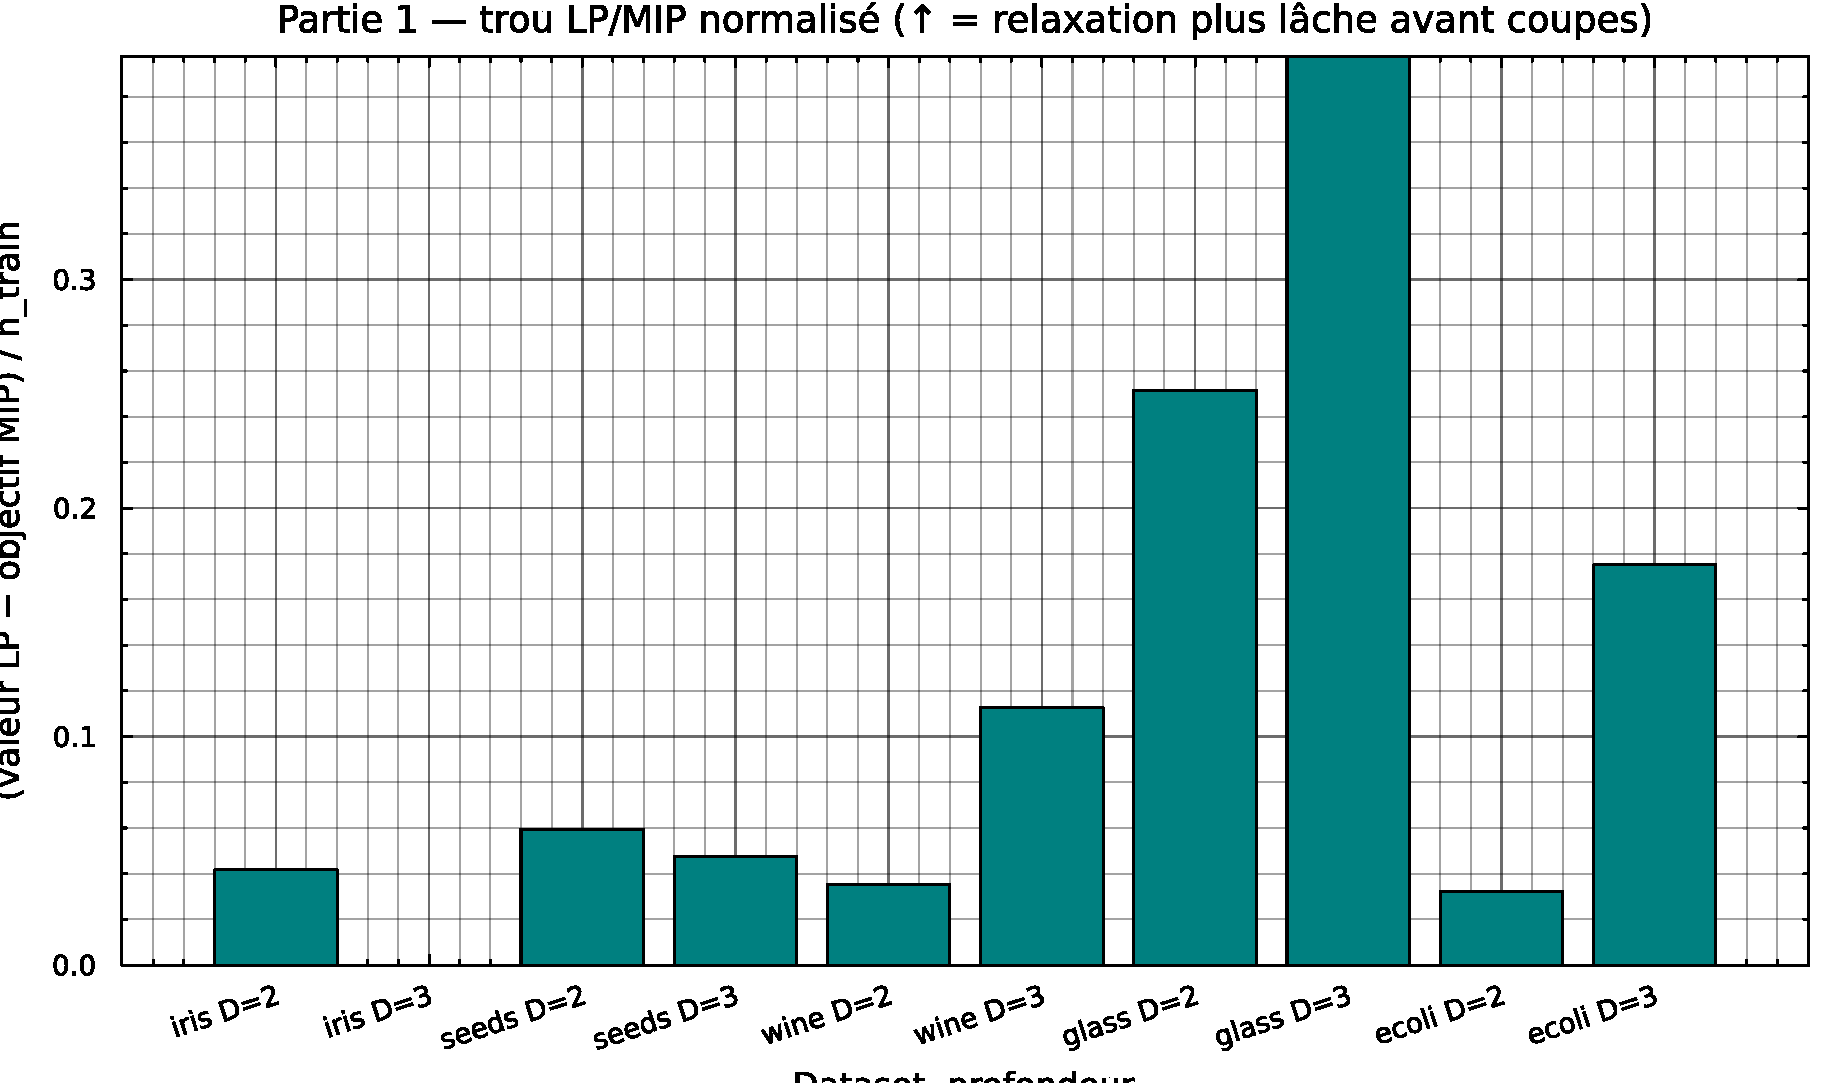
\includegraphics[width=\textwidth]{figures/part1_lp_mip_gap_normalized.pdf}
  \caption{Écart de relaxation $(\text{LP}-\text{MIP})/n_{\text{train}}$ sans égalités.}
\end{subfigure}
\caption{Indicateurs complémentaires pour la Partie~1 (même protocole que la figure~\ref{fig:part1_comparison}).}
\label{fig:part1_enriched}
\end{figure}

\subsection{Analyse}

\begin{resultbox}[Observations clés -- Partie 1]
\begin{itemize}
  \item \textbf{Bilan global (run 300\,s, sans arrondi, $D=2$).} L'ajout d'égalités ne change pas les erreurs test sur les cinq jeux (\texttt{iris} 1, \texttt{seeds} 2, \texttt{wine} 2, \texttt{glass} 17, \texttt{ecoli} 6), ce qui indique une qualité prédictive stable.
  \item \textbf{Impact temps.} L'effet sur le temps de résolution est faible à modéré selon le jeu : amélioration sur \texttt{iris} (1{,}3\,s $\to$ 0{,}9\,s) et \texttt{ecoli} (3{,}1\,s $\to$ 3{,}0\,s), neutre sur \texttt{seeds} (11{,}6\,s $\to$ 11{,}6\,s), légère hausse sur \texttt{wine} (12{,}1\,s $\to$ 12{,}2\,s) et \texttt{glass} (263{,}6\,s $\to$ 264{,}4\,s).
  \item \textbf{Impact B\&B.} Les égalités réduisent les nœuds explorés sur \texttt{iris} (1181 $\to$ 1070) et \texttt{glass} (843168 $\to$ 818825), et sont neutres sur \texttt{seeds}, \texttt{wine} et \texttt{ecoli}.
  \item \textbf{Cas \texttt{glass}.} C'est l'instance la plus coûteuse du lot (ordre de grandeur $10^5$--$10^6$ nœuds), où les égalités apportent un allègement du B\&B mais pas de gain de précision ni de temps net.
  \item Ces résultats suggèrent que, dans ce protocole, les égalités jouent surtout un rôle de \textbf{stabilisation/resserrement de la recherche combinatoire}, avec un bénéfice pratique dépendant du dataset.
\end{itemize}
\end{resultbox}

% ══════════════════════════════════════════════════════════════════════════
% ══════════════════════════════════════════════════════════════════════════
\section{Partie 2 -- Arbres de décision équitables}
\label{sec:part2}
% ══════════════════════════════════════════════════════════════════════════

\subsection{Méthode}

On augmente le modèle MIP (flux unitaire) avec des contraintes d'équité. Chaque échantillon possède un \textbf{attribut sensible} binaire $g(i) \in \{A, B\}$, et on fixe une classe positive $k_{\text{pos}}$. Deux critères sont considérés :

\begin{itemize}
  \item \textbf{Parité démographique} : $P(\hat{y}{=}\text{pos} \mid A) = P(\hat{y}{=}\text{pos} \mid B)$.
  \item \textbf{Equal opportunity} : $\text{TPR}_A = \text{TPR}_B$ (taux de vrais positifs égal entre groupes).
\end{itemize}

\paragraph{Linéarisation.} L'indicatrice $\text{pred}_i = \sum_{t \in \mathcal{L}} u^i_{t,w} \cdot c_{k_{\text{pos}}, t}$ est un produit de variables binaires. On introduit $w_{i,t} \in \{0,1\}$ avec :
\begin{equation}
w_{i,t} \leq u^i_{t,w}, \quad w_{i,t} \leq c_{k_{\text{pos}}, t}, \quad w_{i,t} \geq u^i_{t,w} + c_{k_{\text{pos}}, t} - 1.
\label{eq:linfair}
\end{equation}

Le taux de prédiction positive dans chaque groupe s'exprime alors comme $r_g = \frac{1}{|g|} \sum_{i \in g} \sum_t w_{i,t}$.

\begin{theorybox}[Validité de la linéarisation]

Les trois inégalités~\eqref{eq:linfair} forment une linéarisation exacte du produit $u^i_{t,w} \cdot c_{k_{\text{pos}}, t}$ de deux variables binaires. Montrons que $w_{i,t} = u^i_{t,w} \cdot c_{k_{\text{pos}}, t}$ pour toute solution entière~:

\begin{itemize}
  \item Si $u^i_{t,w} = 0$ : les deux premières inégalités donnent $w_{i,t} \leq 0$, donc $w_{i,t} = 0 = 0 \cdot c_{k_{\text{pos}}, t}$.
  \item Si $c_{k_{\text{pos}}, t} = 0$ : la deuxième inégalité donne $w_{i,t} \leq 0$, donc $w_{i,t} = 0 = u^i_{t,w} \cdot 0$.
  \item Si $u^i_{t,w} = 1$ et $c_{k_{\text{pos}}, t} = 1$ : la troisième inégalité donne $w_{i,t} \geq 1 + 1 - 1 = 1$, donc $w_{i,t} = 1 = 1 \cdot 1$.
\end{itemize}

La contrainte de parité~\eqref{eq:constraint} (ou sa version avec tolérance) est donc bien équivalente à l'égalité des taux de prédiction positive entre groupes pour toute solution entière.
\end{theorybox}

\paragraph{Configurations testées.}

\begin{enumerate}
  \item \textbf{Contrainte stricte} : $r_A = r_B$, linéarisée par mise au même dénominateur~:
  \begin{equation}
    n_B \sum_{i \in A} \sum_{t \in \mathcal{L}} w_{i,t} \;=\; n_A \sum_{i \in B} \sum_{t \in \mathcal{L}} w_{i,t}.
    \label{eq:constraint}
  \end{equation}
  \item \textbf{Tolérance} : $|r_A - r_B| \leq \varepsilon$ avec $\varepsilon = 0{,}15$, modélisée via deux variables de slack $s^+, s^- \geq 0$ telles que $r_A - r_B = s^+ - s^-$ et $s^+ + s^- \leq \varepsilon$.
  \item \textbf{Pénalité} : objectif $\max(\text{accuracy} - \lambda (s^+ + s^-))$ avec $\lambda = 80$, qui favorise l'équité sans la forcer strictement.
\end{enumerate}

\subsection{Résultats expérimentaux}

\paragraph{Protocole.} Cinq jeux de données (iris, seeds, wine, glass, ecoli). Groupe sensible synthétique : médiane de la première feature. Quatre configurations comparées à $D \in \{2,3\}$. Limite CPLEX \texttt{DEFAULT\_TIME\_LIMIT\_PARTS} (typ.\ 300\,s ; les valeurs ci-dessous proviennent de \texttt{part2\_results.csv}). Colonne \textbf{Gap}~: écart d'optimalité MIP (\%) lorsque la limite est atteinte.

\begin{table}[H]
\centering
\caption{Partie 2 -- Compromis équité-précision (parité démographique, $D=2$). Source : \texttt{part2\_results.csv}.}
\label{tab:part2}
\small
\begin{tabular}{@{}l l r r r r r@{}}
\toprule
Dataset & Configuration & Temps (s) & Gap (\%) & Err.\ train & Err.\ test & Parity gap \\
\midrule
\multirow{4}{*}{iris}
 & Sans équité        & 1{,}3  & 0 & 5  & 1  & 0{,}70 \\
 & Contrainte stricte & 7{,}0  & 0 & 43 & 15 & 0{,}00 \\
 & Tolérance 0{,}15   & 6{,}3  & 0 & 34 & 6  & 0{,}15 \\
 & Pénalité $\lambda{=}80$ & 7{,}2  & 0 & 43 & 13 & 0{,}00 \\
\midrule
\multirow{4}{*}{seeds}
 & Sans équité        & 6{,}0  & 0 & 10 & 2 & 0{,}02 \\
 & Contrainte stricte & 205{,}8 & 0 & 53 & 17 & 0{,}00 \\
 & Tolérance 0{,}15   & 9{,}4  & 0 & 10 & 2  & 0{,}02 \\
 & Pénalité $\lambda{=}80$ & 18{,}7 & 0 & 10 & 2  & 0{,}02 \\
\midrule
\multirow{4}{*}{wine}
 & Sans équité        & 9{,}0  & 0 & 5  & 2  & 0{,}60 \\
 & Contrainte stricte & 190{,}6 & 0 & 46 & 13 & 0{,}00 \\
 & Tolérance 0{,}15   & 46{,}4 & 0 & 31 & 12 & 0{,}14 \\
 & Pénalité $\lambda{=}80$ & 50{,}9 & 0 & 39 & 15 & 0{,}01 \\
\midrule
\multirow{4}{*}{glass}
 & Sans équité        & 45{,}1 & 0 & 56 & 16 & 0{,}19 \\
 & Contrainte stricte & 177{,}9 & 0 & 81 & 26 & 0{,}00 \\
 & Tolérance 0{,}15   & 123{,}2 & 0 & 61 & 18 & 0{,}15 \\
 & Pénalité $\lambda{=}80$ & 293{,}4 & 0 & 65 & 21 & 0{,}05 \\
\midrule
\multirow{4}{*}{ecoli}
 & Sans équité        & 3{,}6  & 0 & 7  & 6  & 0{,}56 \\
 & Contrainte stricte & 300{,}0 & 38{,}7 & 105 & 24 & 0{,}00 \\
 & Tolérance 0{,}15   & 23{,}6 & 0 & 45 & 14 & 0{,}15 \\
 & Pénalité $\lambda{=}80$ & 31{,}2 & 0 & 7  & 6  & 0{,}56 \\
\bottomrule
\end{tabular}
\end{table}

\begin{table}[H]
\centering
\caption{Partie 2 -- Même protocole, profondeur $D=3$ (extrait \texttt{part2\_results.csv}). $^\dagger$~gap MIP $>0$ : limite de temps atteinte sans preuve d'optimalité.}
\label{tab:part2d3}
\small
\begin{tabular}{@{}l l r r r r r@{}}
\toprule
Dataset & Configuration & Temps (s) & Gap (\%) & Err.\ train & Err.\ test & Parity gap \\
\midrule
\multirow{4}{*}{iris}
 & Sans équité        & 8{,}4  & 0 & 0 & 4 & 0{,}70 \\
 & Contrainte stricte & 185{,}9 & 0 & 42 & 4 & 0{,}00 \\
 & Tolérance 0{,}15   & 300{,}0$^\dagger$ & 29{,}7 & 33 & 13 & 0{,}15 \\
 & Pénalité $\lambda{=}80$ & 79{,}3 & 0 & 42 & 3 & 0{,}00 \\
\midrule
\multirow{4}{*}{seeds}
 & Sans équité        & 300{,}7$^\dagger$ & 3{,}7 & 6 & 1 & 0{,}04 \\
 & Contrainte stricte & 300{,}0$^\dagger$ & 46{,}1 & 53 & 17 & 0{,}00 \\
 & Tolérance 0{,}15   & 301{,}4$^\dagger$ & 1{,}8 & 3 & 1 & 0{,}03 \\
 & Pénalité $\lambda{=}80$ & 300{,}1$^\dagger$ & 4{,}7 & 6 & 3 & 0{,}02 \\
\midrule
\multirow{4}{*}{wine}
 & Sans équité        & 40{,}9 & 0 & 0 & 6 & 0{,}55 \\
 & Contrainte stricte & 300{,}0$^\dagger$ & 51{,}1 & 48 & 15 & 0{,}00 \\
 & Tolérance 0{,}15   & 300{,}0$^\dagger$ & 25{,}7 & 29 & 10 & 0{,}15 \\
 & Pénalité $\lambda{=}80$ & 300{,}0$^\dagger$ & 38{,}5 & 39 & 9 & 0{,}01 \\
\midrule
\multirow{4}{*}{glass}
 & Sans équité        & 300{,}0$^\dagger$ & 23{,}6 & 37 & 14 & 0{,}19 \\
 & Contrainte stricte & 300{,}0$^\dagger$ & 90{,}0 & 81 & 23 & 0{,}00 \\
 & Tolérance 0{,}15   & 300{,}0$^\dagger$ & 36{,}8 & 46 & 14 & 0{,}09 \\
 & Pénalité $\lambda{=}80$ & 300{,}0$^\dagger$ & 47{,}1 & 53 & 17 & 0{,}03 \\
\midrule
\multirow{4}{*}{ecoli}
 & Sans équité        & 300{,}0$^\dagger$ & 0{,}9 & 3 & 5 & 0{,}58 \\
 & Contrainte stricte & 300{,}1$^\dagger$ & 93{,}7 & 105 & 24 & 0{,}00 \\
 & Tolérance 0{,}15   & 300{,}1$^\dagger$ & 24{,}7 & 43 & 11 & 0{,}15 \\
 & Pénalité $\lambda{=}80$ & 300{,}1$^\dagger$ & 29{,}2 & 3 & 5 & 0{,}58 \\
\bottomrule
\end{tabular}
\end{table}

\begin{figure}[H]
\centering
\begin{subfigure}[t]{0.48\textwidth}
  \centering
  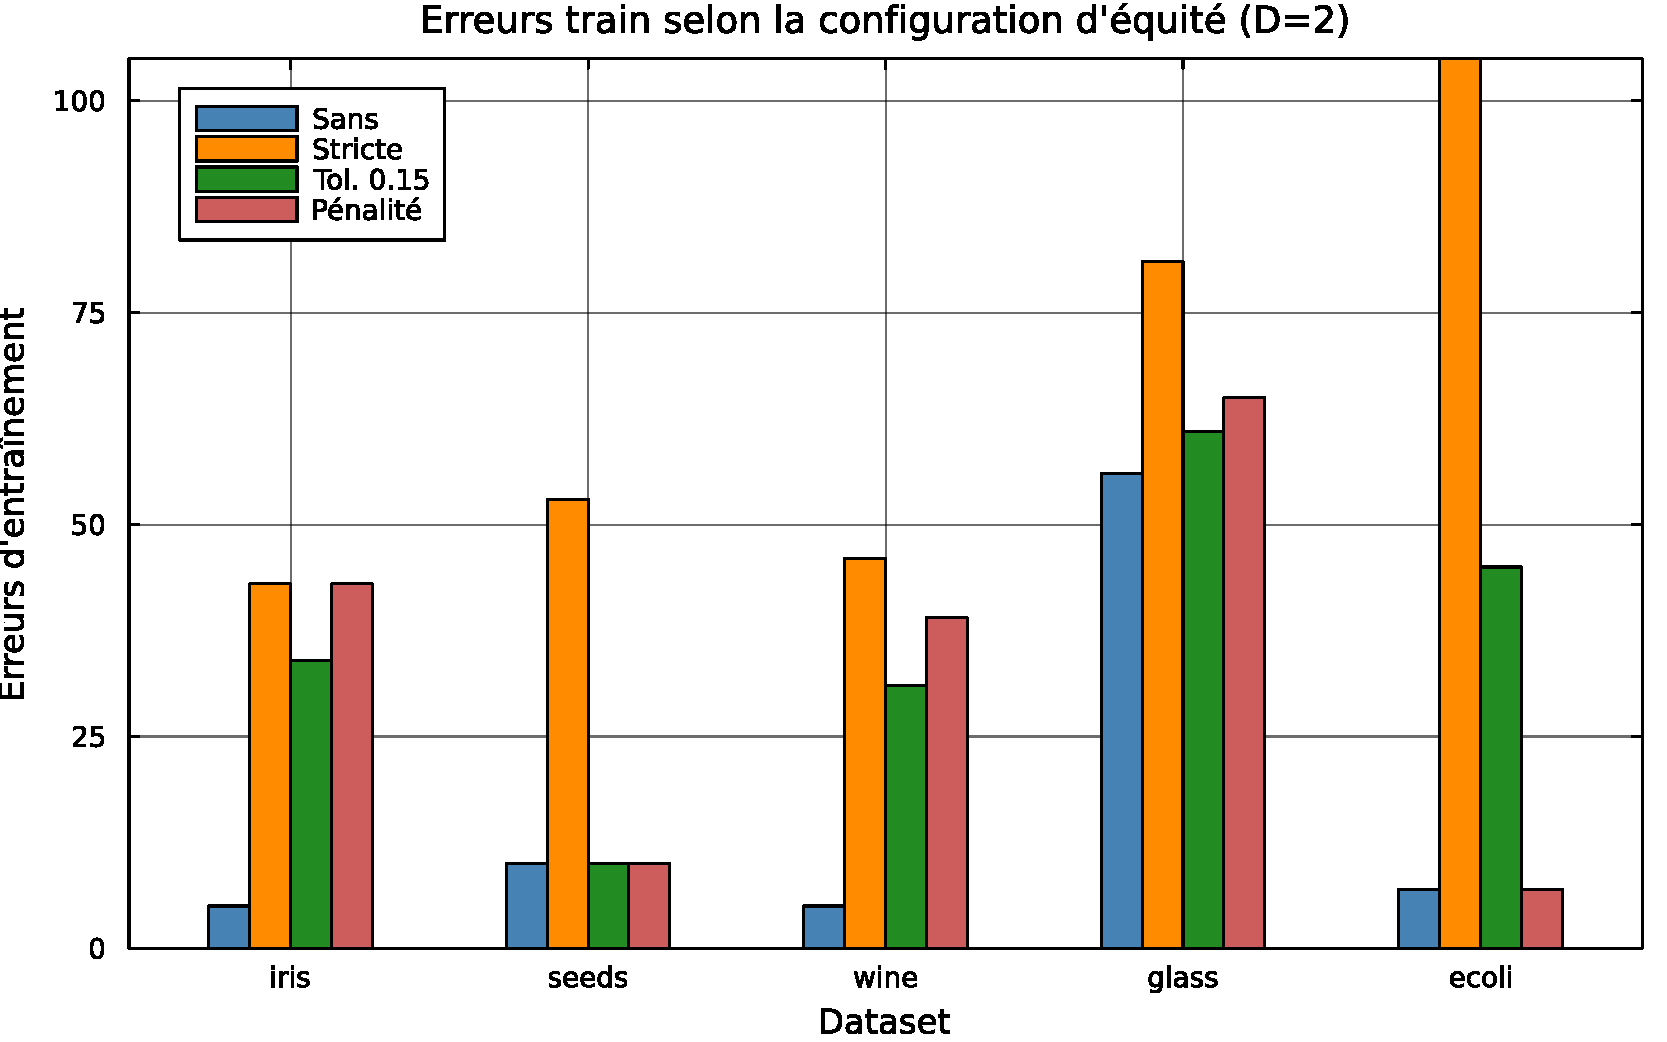
\includegraphics[width=\textwidth]{figures/part2_accuracy_vs_fairness.pdf}
  \caption{Erreurs d'entraînement.}
\end{subfigure}
\hfill
\begin{subfigure}[t]{0.48\textwidth}
  \centering
  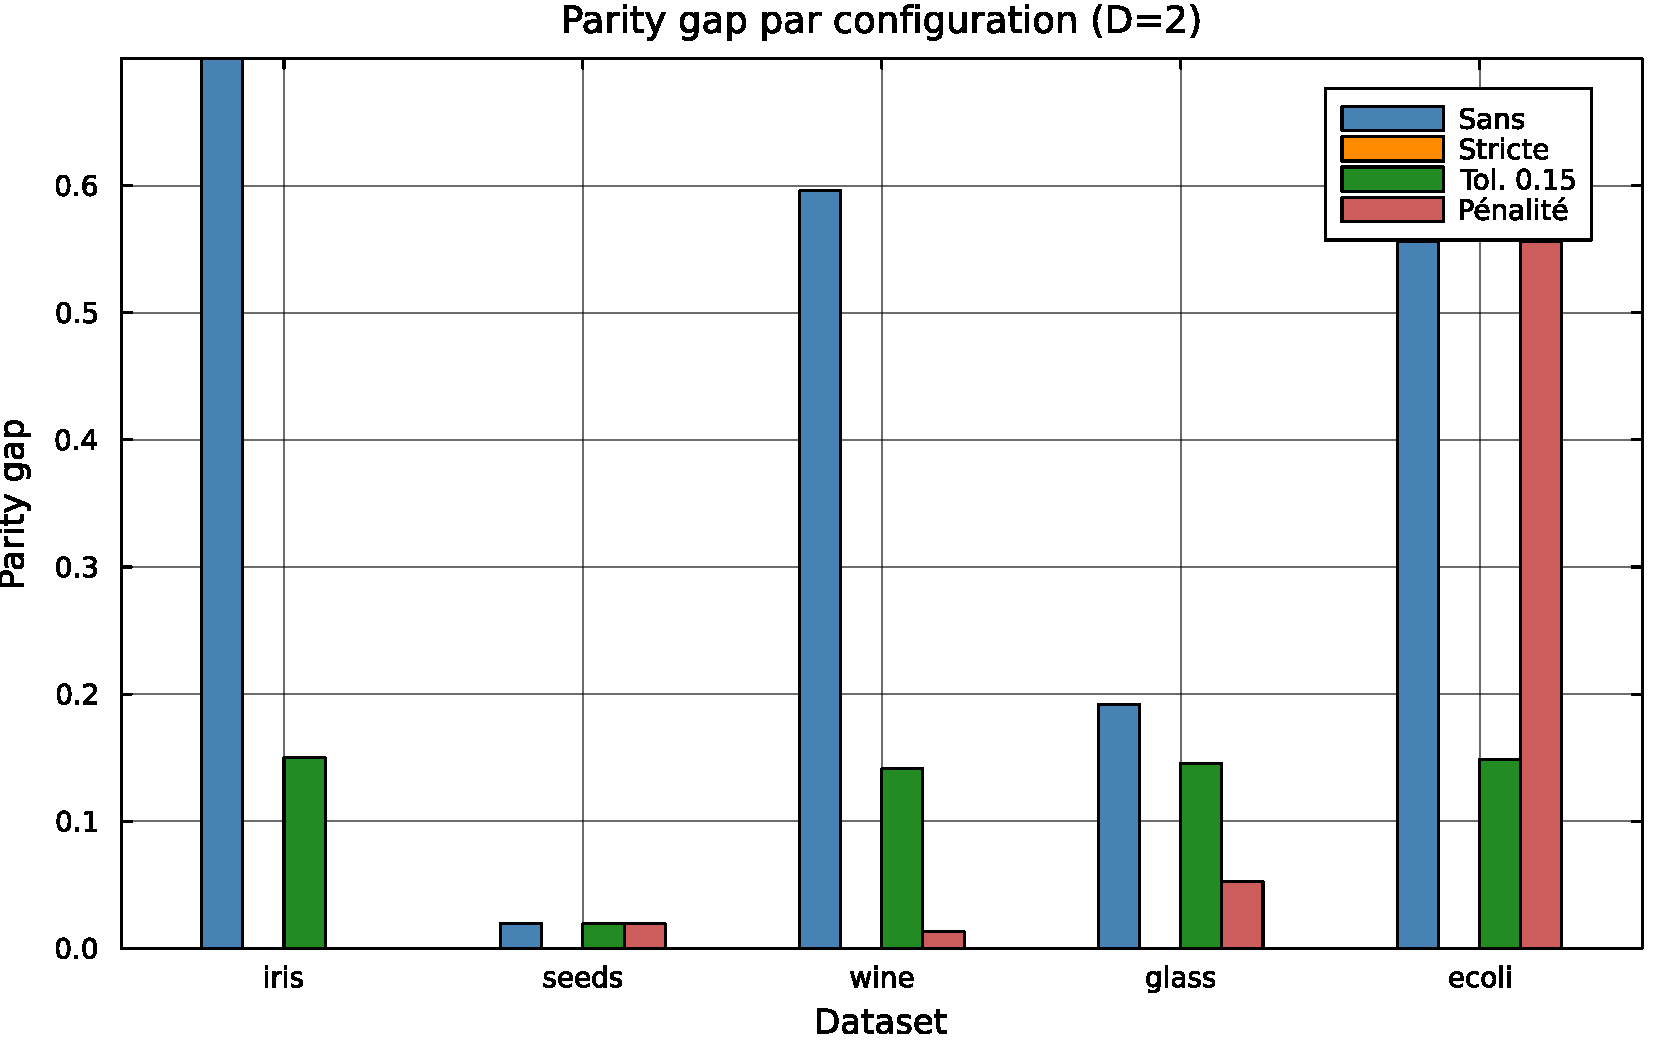
\includegraphics[width=\textwidth]{figures/part2_parity_gap.pdf}
  \caption{Parity gap résiduel.}
\end{subfigure}
\caption{Impact des contraintes d'équité sur la précision et le parity gap ($D=2$).}
\label{fig:part2}
\end{figure}

\begin{figure}[H]
\centering
\begin{subfigure}[t]{0.48\textwidth}
  \centering
  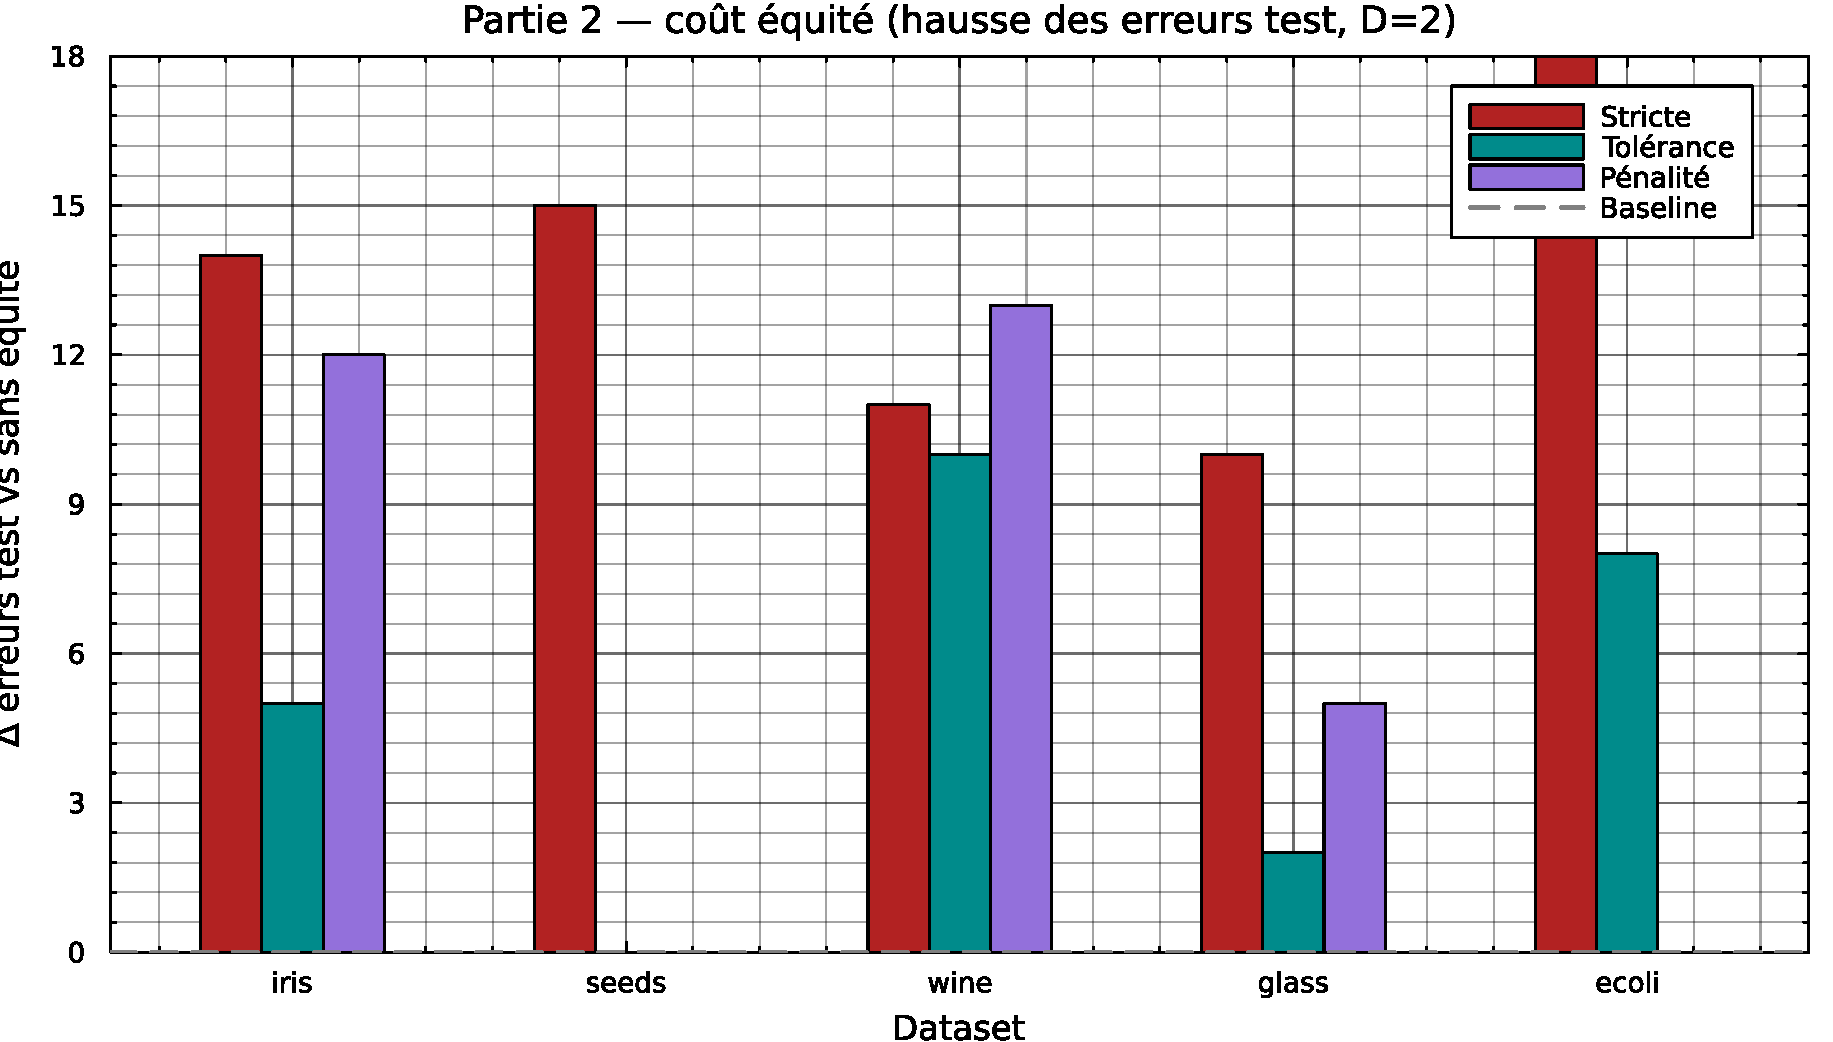
\includegraphics[width=\textwidth]{figures/part2_fairness_cost_delta_test_D2.pdf}
  \caption{$\Delta$ erreurs test vs sans équité ($D=2$).}
\end{subfigure}
\hfill
\begin{subfigure}[t]{0.48\textwidth}
  \centering
  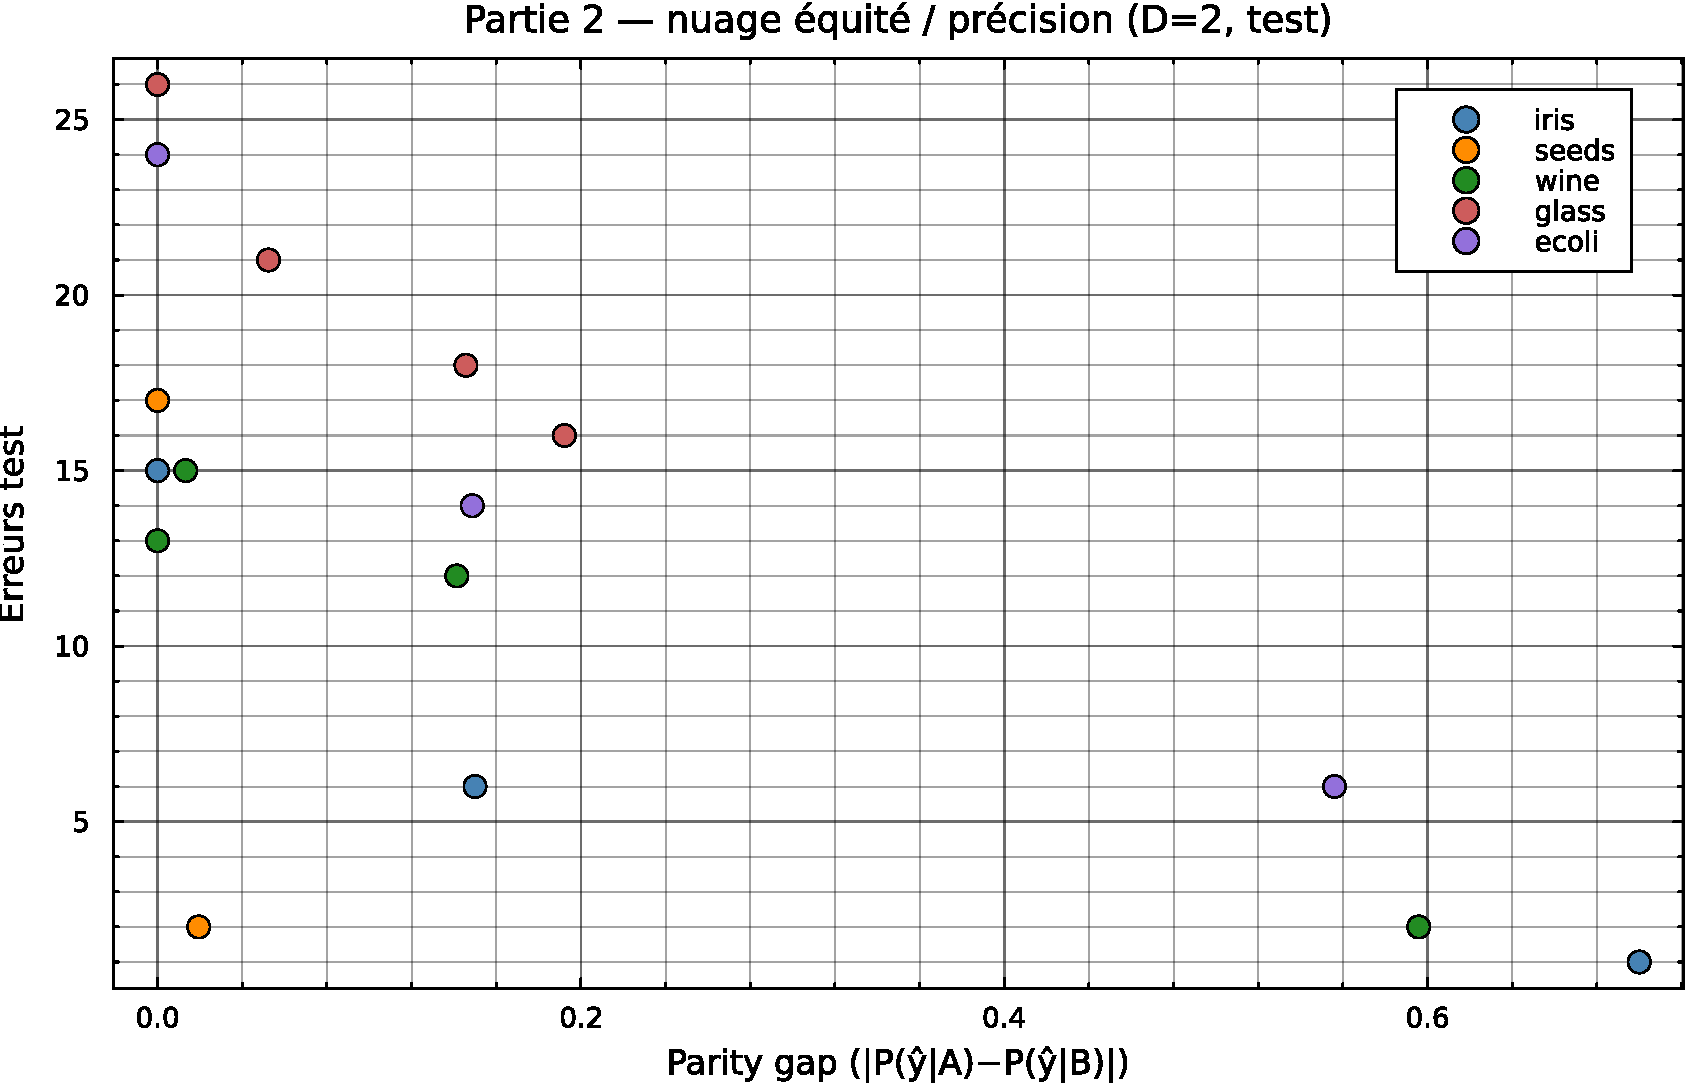
\includegraphics[width=\textwidth]{figures/part2_fairness_tradeoff_paths_D2.pdf}
  \caption{Nuage de points dans l'espace (parity gap, erreurs test).}
\end{subfigure}
\caption{Figures complémentaires Partie~2 (même CSV que les tableaux~\ref{tab:part2}--\ref{tab:part2d3}).}
\label{fig:part2_enriched}
\end{figure}

\begin{figure}[H]
\centering
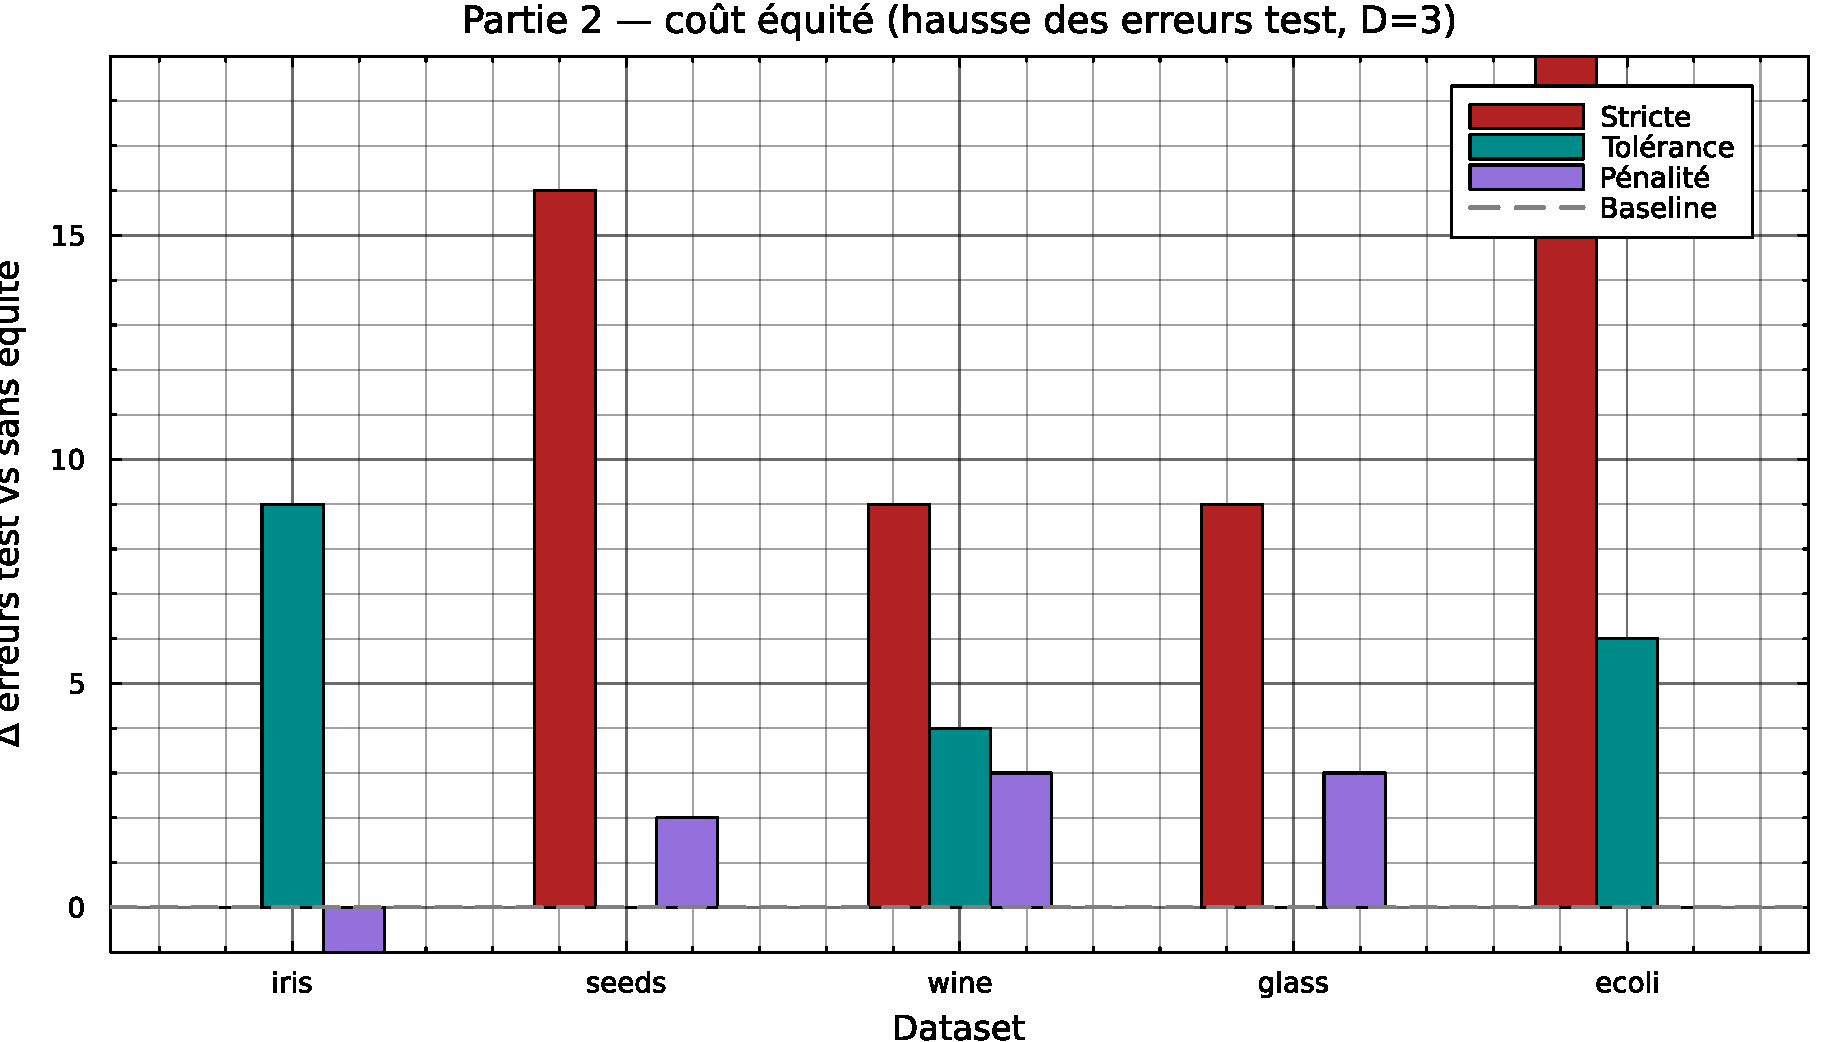
\includegraphics[width=0.72\textwidth]{figures/part2_fairness_cost_delta_test_D3.pdf}
\caption{$\Delta$ erreurs test vs configuration sans équité pour $D{=}3$ (tableau~\ref{tab:part2d3}).}
\label{fig:part2_delta_d3}
\end{figure}

\subsection{Analyse}

\begin{resultbox}[Observations clés -- Partie 2]
\begin{itemize}
  \item Le compromis équité--précision est confirmé par \texttt{part2\_results.csv} : la contrainte stricte force un parity gap nul, mais augmente fortement les erreurs (ex.\ à $D{=}2$ : \texttt{iris} 5 $\to$ 43 train et 1 $\to$ 15 test ; \texttt{wine} 5 $\to$ 46 train et 2 $\to$ 13 test).
  \item \textbf{Seeds} a un gap initial faible (0{,}019 à $D{=}2$) : tolérance et pénalité gardent pratiquement le même niveau d'équité et la même précision (10 erreurs train, 2 test).
  \item \textbf{Tolérance $\varepsilon=0{,}15$} : à $D{=}2$, c'est le meilleur compromis sur les jeux avec gap initial élevé (\texttt{iris}, \texttt{wine}, \texttt{glass}, \texttt{ecoli}), avec un coût en erreurs inférieur à la contrainte stricte et des temps nettement plus bas.
  \item \textbf{Pénalité} : comportement dataset-dépendant. Elle fonctionne bien sur \texttt{iris} et \texttt{wine} (gap proche de 0), mais peut échouer à réduire l'inéquité sur \texttt{ecoli} ($D{=}2$ : parity gap inchangé à 0{,}556, mêmes erreurs que sans équité).
  \item À $D{=}3$, plusieurs configurations atteignent 300\,s avec \textbf{gap MIP non nul} (\texttt{seeds}, \texttt{wine}, \texttt{glass}, \texttt{ecoli}) ; les métriques rapportées sont donc celles de la meilleure solution trouvée, sans preuve d'optimalité entière.
  \item \textbf{Glass} et \textbf{ecoli} restent les cas les plus difficiles : la contrainte stricte y est très coûteuse (ex.\ \texttt{ecoli} $D{=}3$ : gap 93{,}7\,\%, 105 erreurs train, 24 test).
\end{itemize}
\end{resultbox}


% ══════════════════════════════════════════════════════════════════════════
% ══════════════════════════════════════════════════════════════════════════
\section{Partie 3 -- Features dérivées}
\label{sec:part3}
% ══════════════════════════════════════════════════════════════════════════

\subsection{Méthode}

L'idée est d'améliorer la classification en ajoutant de nouvelles features calculées à partir des features existantes, tout en conservant des expressions simples pour l'interprétabilité. L'algorithme procède en quatre étapes :

\begin{enumerate}
  \item \textbf{Génération des candidats.} Pour chaque paire de features $(j_1, j_2)$, on calcule trois combinaisons algébriques : $x_{j_1} / (x_{j_2} + \varepsilon)$, $x_{j_1} - x_{j_2}$, $x_{j_1} \times x_{j_2}$. Cela produit au plus $3 p(p-1)$ candidats pour $p$ features.
  \item \textbf{Scoring par gain de Gini.} Chaque candidat est évalué par le gain de Gini du meilleur split binaire sur cette colonne (seuil optimal parmi les midpoints entre valeurs triées).
  \item \textbf{Sélection des top-$k$.} Les $k$ candidats de plus grand gain sont retenus (par défaut $k{=}5$). Les paramètres des features (indices, type) sont stockés pour pouvoir appliquer la même transformation au jeu de test.
  \item \textbf{Normalisation.} Après concaténation, les nouvelles colonnes sont normalisées dans $[0,1]$ avec les min/max de l'entraînement.
\end{enumerate}

\subsection{Résultats expérimentaux}

\paragraph{Protocole.} Cinq jeux (iris, seeds, wine, glass, ecoli). Pour chaque couple (dataset, $D$), comparaison sans nouvelles colonnes vs avec $k{=}5$ features dérivées. Limite CPLEX \texttt{DEFAULT\_TIME\_LIMIT\_PARTS} (référence : \texttt{part3\_results.csv}). Colonne \textbf{Gap} : écart d'optimalité MIP (\%) si la limite est atteinte. $n_{\text{spl}}$ : nombre de splits de l'arbre (structure fixée par $D$).

\begin{table}[H]
\centering
\caption{Partie 3 -- Impact des features dérivées sur la précision et le temps (source \texttt{part3\_results.csv}).}
\label{tab:part3}
\small
\begin{tabular}{@{}l c l r r r r r r@{}}
\toprule
Dataset & $D$ & Config & Temps (s) & Gap (\%) & Obj. & Err.\ tr. & Err.\ te. & $n_{\text{feat}}$ / $n_{\text{spl}}$ \\
\midrule
\multirow{2}{*}{iris} & \multirow{2}{*}{2} & Sans & 0{,}6 & 0 & 115 & 5 & 1 & 4 / 3 \\
 & & Avec & 1{,}8 & 0 & 115 & 5 & 1 & 9 / 3 \\
\cmidrule{2-9}
\multirow{2}{*}{} & \multirow{2}{*}{3} & Sans & 8{,}5 & 0 & 120 & 0 & 4 & 4 / 7 \\
 & & Avec & 8{,}3 & 0 & 120 & 0 & \cellcolor{navylight}\textbf{3} & 9 / 7 \\
\midrule
\multirow{2}{*}{seeds} & \multirow{2}{*}{2} & Sans & 6{,}2 & 0 & 158 & 10 & 2 & 6 / 3 \\
 & & Avec & 7{,}7 & 0 & 158 & 10 & 2 & 11 / 3 \\
\cmidrule{2-9}
\multirow{2}{*}{} & \multirow{2}{*}{3} & Sans & 300{,}9 & 3{,}7 & 162 & 6 & 1 & 6 / 7 \\
 & & Avec & 301{,}1 & 2{,}4 & 164 & 7 & 4 & 11 / 7 \\
\midrule
\multirow{2}{*}{wine} & \multirow{2}{*}{2} & Sans & 8{,}3 & 0 & 137 & 5 & 2 & 13 / 3 \\
 & & Avec & 8{,}5 & 0 & 140 & \cellcolor{navylight}\textbf{2} & \cellcolor{navylight}\textbf{1} & 18 / 3 \\
\cmidrule{2-9}
\multirow{2}{*}{} & \multirow{2}{*}{3} & Sans & 37{,}3 & 0 & 142 & 0 & 6 & 13 / 7 \\
 & & Avec & 11{,}7 & 0 & 142 & 0 & \cellcolor{navylight}\textbf{4} & 18 / 7 \\
\midrule
\multirow{2}{*}{glass} & \multirow{2}{*}{2} & Sans & 45{,}5 & 0 & 115 & 56 & 16 & 9 / 3 \\
 & & Avec & 48{,}2 & 0 & 116 & 55 & 16 & 14 / 3 \\
\cmidrule{2-9}
\multirow{2}{*}{} & \multirow{2}{*}{3} & Sans & 300{,}0 & 30{,}2 & 130 & 41 & 16 & 9 / 7 \\
 & & Avec & 300{,}9 & 33{,}9 & 127 & 44 & 20 & 14 / 7 \\
\midrule
\multirow{2}{*}{ecoli} & \multirow{2}{*}{2} & Sans & 3{,}2 & 0 & 210 & 7 & 6 & 7 / 3 \\
 & & Avec & 7{,}7 & 0 & 210 & 7 & 6 & 12 / 3 \\
\cmidrule{2-9}
\multirow{2}{*}{} & \multirow{2}{*}{3} & Sans & 300{,}1 & 0{,}9 & 214 & 3 & 5 & 7 / 7 \\
 & & Avec & 301{,}4 & 1{,}9 & 213 & 4 & 6 & 12 / 7 \\
\bottomrule
\end{tabular}
\end{table}

\begin{figure}[H]
\centering
\begin{subfigure}[t]{0.48\textwidth}
  \centering
  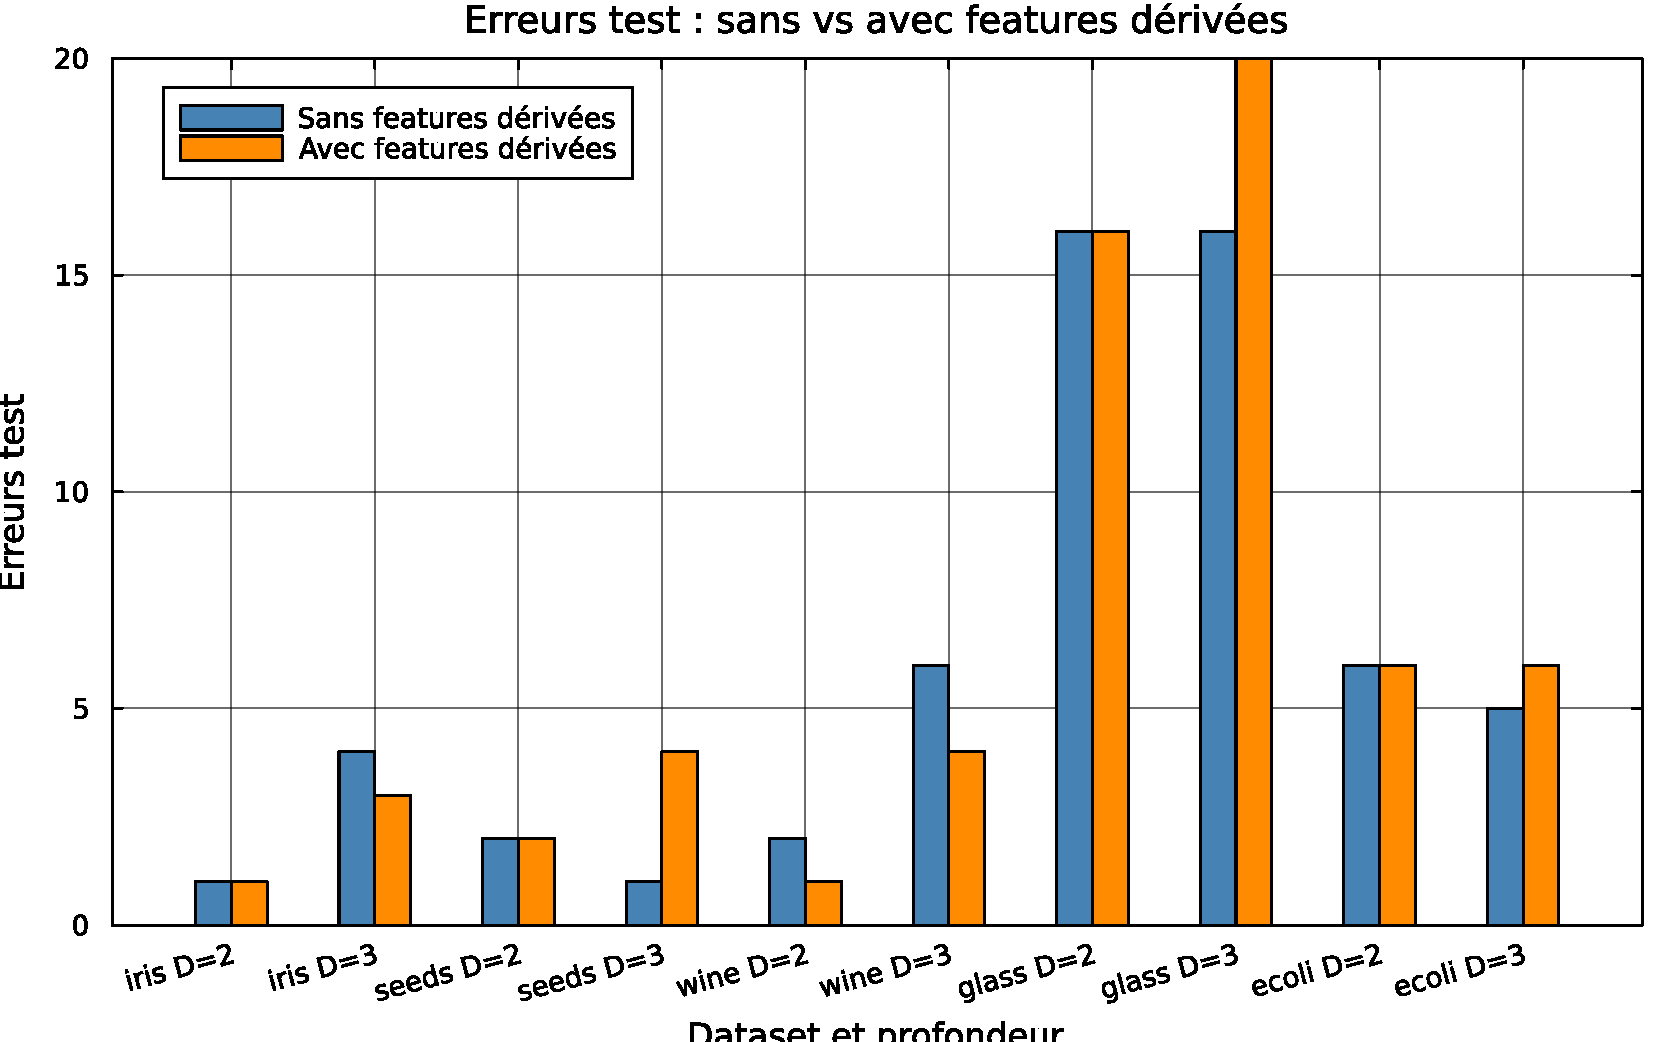
\includegraphics[width=\textwidth]{figures/part3_errors_comparison.pdf}
  \caption{Erreurs test.}
\end{subfigure}
\hfill
\begin{subfigure}[t]{0.48\textwidth}
  \centering
  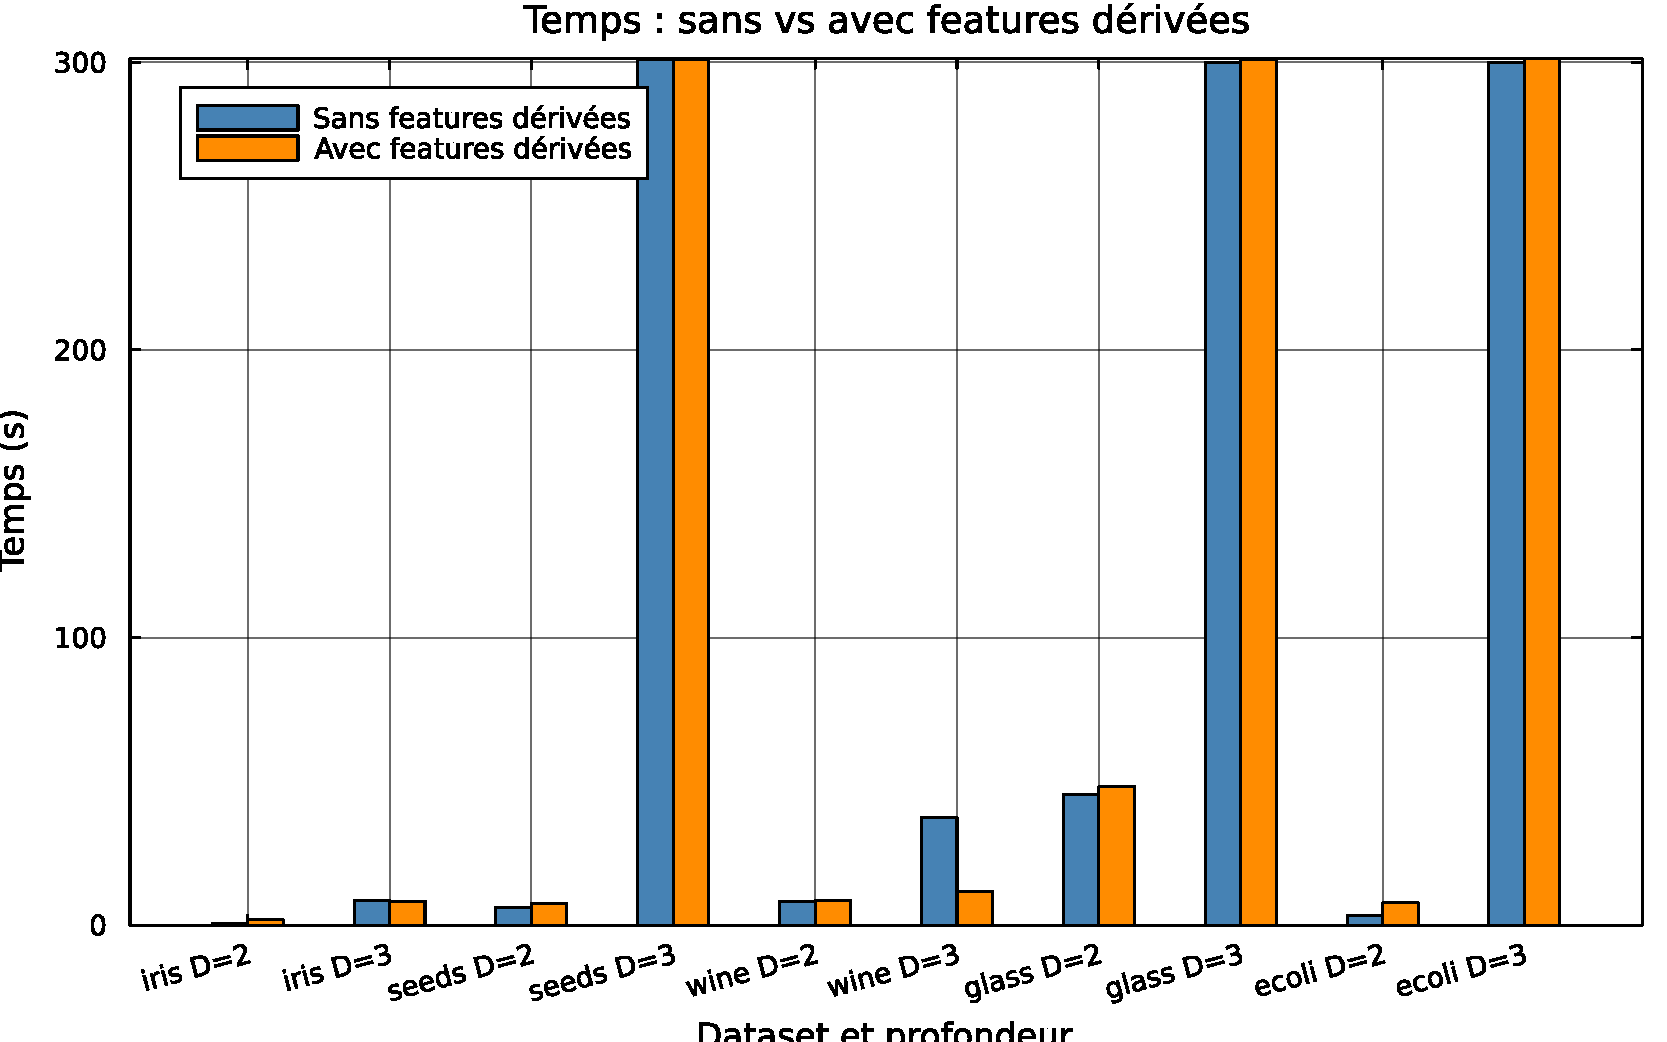
\includegraphics[width=\textwidth]{figures/part3_time_comparison.pdf}
  \caption{Temps de résolution.}
\end{subfigure}
\caption{Comparaison sans vs avec features dérivées pour chaque dataset et profondeur.}
\label{fig:part3}
\end{figure}

\begin{figure}[H]
\centering
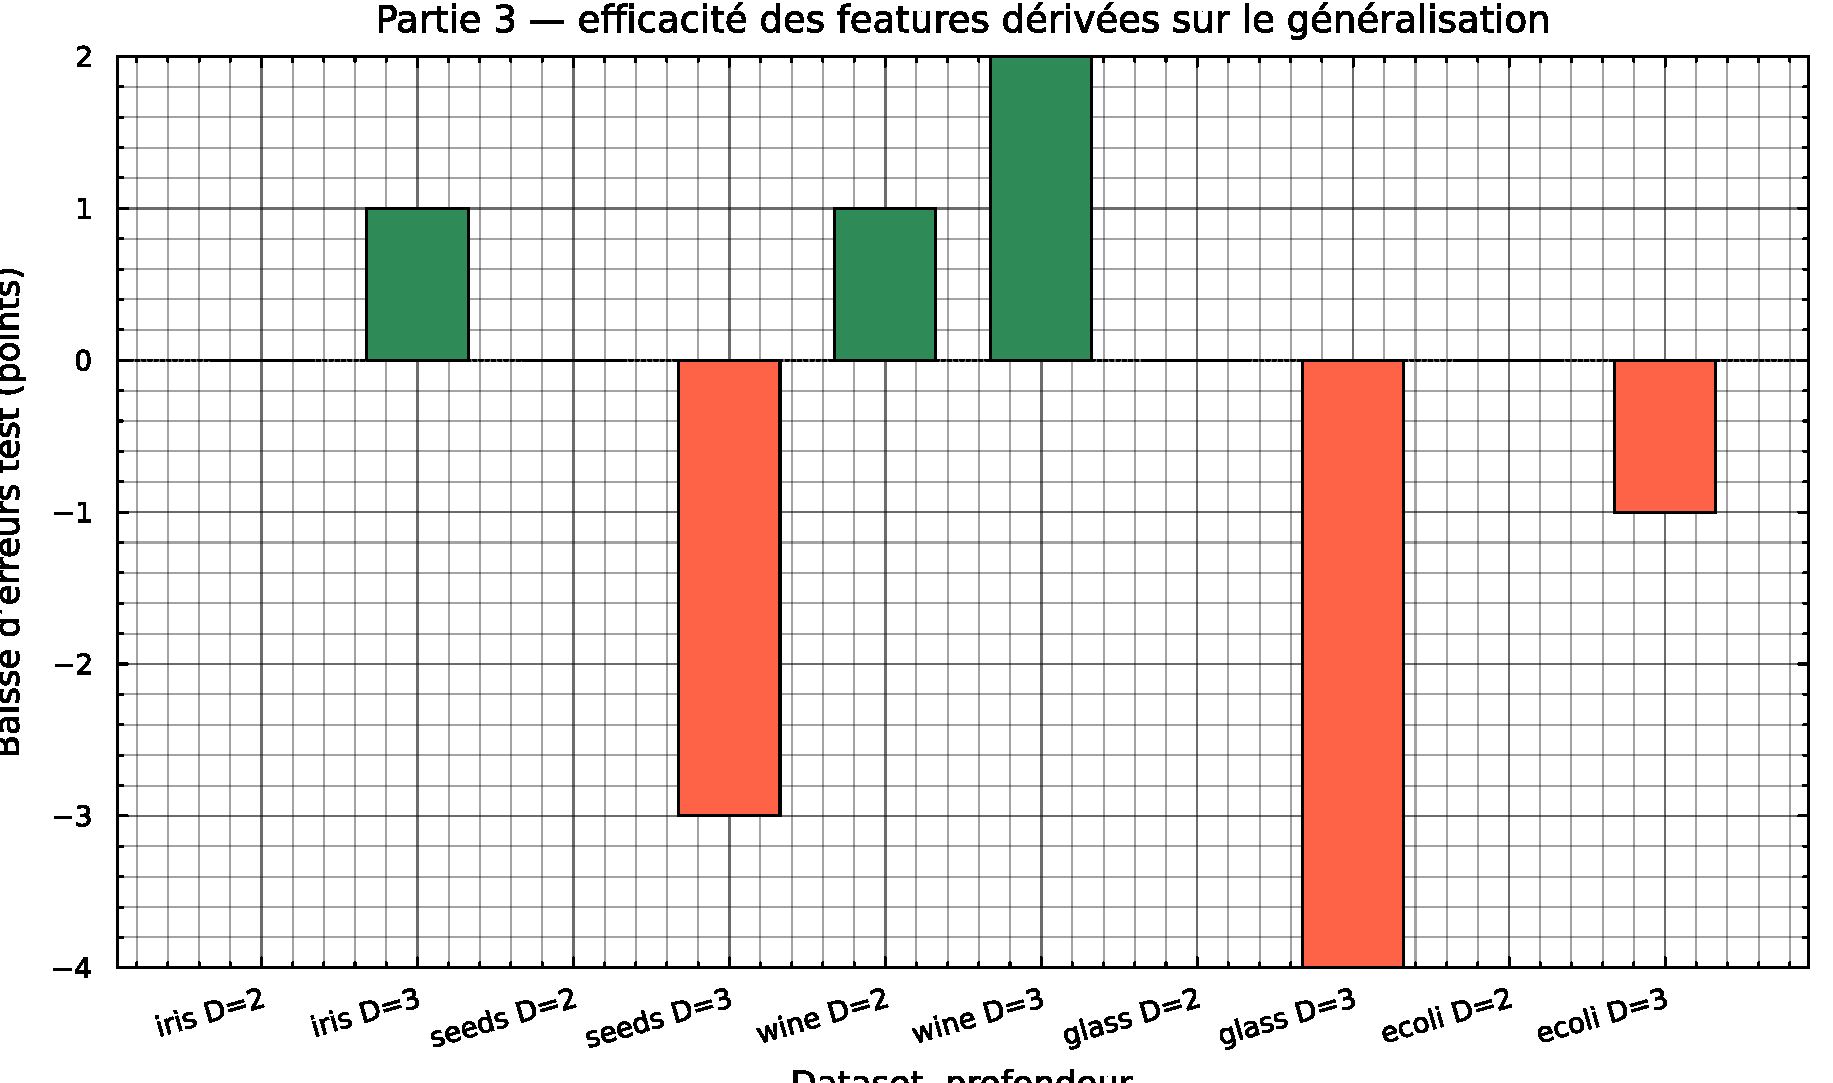
\includegraphics[width=0.72\textwidth]{figures/part3_test_error_delta_features.pdf}
\caption{Écart d'erreurs test (avec $-$ sans features dérivées), par jeu et profondeur (\texttt{part3\_results.csv}).}
\label{fig:part3_delta}
\end{figure}

\subsection{Analyse}

\begin{resultbox}[Observations clés -- Partie 3]
\begin{itemize}
  \item \textbf{Wine} à $D{=}2$ : gain net sur l'entraînement (5 $\to$ 2 erreurs) et sur le test (2 $\to$ 1), à temps comparable. À $D{=}3$, objectif optimal 142 atteint plus vite avec dérivées (12\,s vs 37\,s) et erreurs test 6 $\to$ 4.
  \item \textbf{Iris} à $D{=}3$ : légère amélioration du test (4 $\to$ 3) à objectif et temps comparables ($\sim$8\,s).
  \item \textbf{Seeds} à $D{=}2$ : pas de différence de précision ; à $D{=}3$, les deux runs touchent la limite de temps avec gap MIP ; les dérivées dégradent alors le test (1 $\to$ 4 erreurs) malgré un objectif MIP légèrement différent --- le surdimensionnement de l'espace de recherche peut nuire sous contrainte de temps.
  \item Le \textbf{nombre de splits} est imposé par $D$ ($2^D{-}1$) ; les gains viennent du choix de seuils / features dans un espace de colonnes enrichi.
  \item \textbf{Glass} à $D{=}3$ : sans et avec dérivées atteignent la limite avec fort gap ; les dérivées n'améliorent pas ici le test (16 $\to$ 20 erreurs dans notre tirage).
  \item \textbf{Ecoli} : à $D{=}2$ pas d'effet ; à $D{=}3$ sous limite de temps, légère dégradation (5 $\to$ 6 erreurs test) avec les dérivées.
\end{itemize}
\end{resultbox}


% ══════════════════════════════════════════════════════════════════════════
% ══════════════════════════════════════════════════════════════════════════
\section{Partie 4 -- Formulation univariée pour jeux binaires}
\label{sec:part4}
% ══════════════════════════════════════════════════════════════════════════

\subsection{Section 5.1 : la formulation}

On implémente la formulation spécialisée pour les jeux de données à features binaires ($x_{if} \in \{0,1\}$). L'arbre a des nœuds internes $\mathcal{N} = \{1, \ldots, 2^D{-}1\}$ et des feuilles $\mathcal{L} = \{2^D, \ldots, 2^{D+1}{-}1\}$.

\paragraph{Variables.}
$b_{nf} \in \{0,1\}$ (nœud $n$ branche sur feature $f$),
$p_n \in \{0,1\}$ (nœud $n$ est feuille),
$w_{nk} \in \{0,1\}$ (nœud $n$ prédit classe $k$),
$\theta_i \in \{0,1\}$ (échantillon $i$ bien classé).

\paragraph{Objectif.} $\displaystyle\max\ \frac{1}{|\mathcal{I}|}\sum_{i} \theta_i - \lambda \sum_{n} p_n$.

\paragraph{Convention de branchement.} Si le nœud $n$ branche sur la feature $f$ : le fils gauche ($2n$) reçoit les points avec $x_{if}=0$, le fils droit ($2n+1$) ceux avec $x_{if}=1$.

\begin{theorybox}[Rôle des contraintes (2a)--(2i)]

\textbf{(2a) Objectif.} $\displaystyle\max\ \frac{1}{|\mathcal{I}|}\sum_{i \in \mathcal{I}} \theta_i - \lambda \sum_{n \in \mathcal{N}} p_n$. Le premier terme mesure l'accuracy fractionnaire ; le second pénalise la complexité de l'arbre (nombre de feuilles internes) avec un coefficient $\lambda$ petit, ce qui favorise les arbres élagués à précision égale.

\medskip

\textbf{(2b) Structure de l'arbre.} Pour chaque nœud interne $n \in \mathcal{N}$~:
\[
  \sum_{f \in \mathcal{J}} b_{nf} + p_n + \sum_{n_a \in A(n)} p_{n_a} = 1,
\]
où $A(n)$ désigne l'ensemble des ancêtres stricts de $n$. Cette contrainte impose une partition exacte en trois cas mutuellement exclusifs~: soit $n$ branche activement sur une feature ($\sum_f b_{nf} = 1$), soit $n$ est lui-même une feuille ($p_n = 1$), soit un ancêtre de $n$ est déjà une feuille ($\exists\, n_a \in A(n),\; p_{n_a} = 1$), auquel cas le sous-arbre sous $n_a$ est élagué.

\medskip

\textbf{(2c) Prédiction de classe.} Pour chaque nœud $n \in \mathcal{N} \cup \mathcal{L}$~:
\[
  \sum_{k \in K} w_{nk} = p_n.
\]
Si $n$ est une feuille active ($p_n = 1$), il prédit exactement une classe. Si $n$ n'est pas une feuille ($p_n = 0$), alors $w_{nk} = 0$ pour tout $k$ (pas de prédiction).

\medskip

\textbf{(2d) Borne supérieure sur $\theta_i$ pour les nœuds internes.} Pour chaque échantillon $i \in \mathcal{I}$ et chaque nœud interne $n_\ell \in \mathcal{N}$~:
\[
  \theta_i \;\leq\; \underbrace{\sum_{n_a \in AL(n_\ell)} \sum_{\substack{f:\, x_{if}=1}} b_{n_a f} \;+\; \sum_{n_a \in AR(n_\ell)} \sum_{\substack{f:\, x_{if}=0}} b_{n_a f}}_{\text{wrong turns (déviations du chemin)}} \;+\; \underbrace{\sum_{f \in \mathcal{J}} b_{n_\ell f}}_{\text{$n_\ell$ branche}} \;+\; \underbrace{\sum_{n' \in A^+(n_\ell)} w_{n', y_i}}_{\text{prédiction correcte}}
\]
où $AL(n_\ell)$ (resp.\ $AR(n_\ell)$) est l'ensemble des ancêtres de $n_\ell$ pour lesquels le chemin vers $n_\ell$ passe par le fils gauche (resp.\ droit), et $A^+(n_\ell) = A(n_\ell) \cup \{n_\ell\}$. Les \emph{wrong turns} comptent, pour chaque ancêtre sur le chemin, le nombre de features qui enverraient $i$ du mauvais côté~: si $n_a$ est un ancêtre-gauche et $n_a$ branche sur $f$ avec $x_{if} = 1$, alors $i$ aurait dû aller à droite (déviation). Lorsque $i$ suit exactement le chemin jusqu'à $n_\ell$ sans déviation, les termes de wrong turns sont tous nuls ; $\theta_i = 1$ n'est alors possible que si $n_\ell$ est un nœud de branchement actif \emph{ou} si un nœud de $A^+(n_\ell)$ prédit la classe correcte $y_i$ de~$i$.

\medskip

\textbf{(2e) Borne supérieure sur $\theta_i$ pour les feuilles structurelles.} Pour $n_\ell \in \mathcal{L}$ (nœud feuille dans la structure de l'arbre complet), la contrainte est identique à (2d) mais \emph{sans} le terme $\sum_f b_{n_\ell f}$ (une feuille ne branche pas). Ainsi, $\theta_i = 1$ à la feuille $n_\ell$ exige l'absence de déviations sur le chemin \emph{et} une prédiction correcte par un nœud de $A^+(n_\ell)$.

\medskip

\textbf{(2f)--(2i) Domaines.} $b_{nf}, p_n, w_{nk} \in \{0,1\}$ et $\theta_i \in [0,1]$ (relâché en continu, l'intégralité étant forcée par la structure des autres contraintes).
\end{theorybox}

Pour les jeux non binaires, on applique une \textbf{binarisation par seuil médian} : $x_{ij}^{\text{bin}} = \mathbf{1}[x_{ij} \geq \text{médiane}(X_j)]$.

\subsection{Section 5.2 : renforcement par Equivalent Sets}

\begin{theorybox}[Définition : Equivalent Set (ES)]
\begin{definition}
Un ES pour $\bar{J} \subseteq J$ est un sous-ensemble $\bar{I} \subseteq I$ dont tous les éléments ont la même valeur sur les features de $\bar{J}$, mais ne sont pas tous de la même classe. L'arbre ne peut donc pas les séparer en branchant uniquement sur les features de $\bar{J}$.
\end{definition}
\end{theorybox}

On ajoute des variables auxiliaires $\beta_{n,\bar{I}}$ (le sous-arbre en $n$ sépare $\bar{I}$) et $G_k$ (tous les points de classe $k$ dans $\bar{I}$ sont bien classés), avec les contraintes du système~(4).

\begin{theorybox}[Q1 -- Rôle des contraintes du système (4)]

Le système (4) ajoute, pour chaque ES $(\bar{I}, \bar{J})$, des variables auxiliaires $\beta_{n,\bar{I}} \in [0,1]$ (indicatrice~: le sous-arbre enraciné en $n$ \emph{sépare} les échantillons de $\bar{I}$ vers des feuilles différentes), $\beta_{n,l,\bar{I}}$ et $\beta_{n,r,\bar{I}}$ (les éléments de $\bar{I}$ passent tous à gauche / à droite en $n$, puis sont séparés plus bas), et $G_k \in [0,1]$ (tous les éléments de classe $k$ dans $\bar{I}$ sont bien classés). Détaillons chaque contrainte~:

\medskip

\textbf{Contrainte de séparation récursive.}
\[
  \beta_{n,\bar{I}} \;\leq\; \sum_{f \in \bar{J}} b_{nf} \;+\; \beta_{n,l,\bar{I}} \;+\; \beta_{n,r,\bar{I}}.
\]
Le sous-arbre en $n$ sépare $\bar{I}$ ($\beta_{n,\bar{I}} = 1$) seulement dans l'un des cas suivants~: (a)~$n$ branche sur une feature $f \in \bar{J}$, c'est-à-dire une feature sur laquelle les éléments de $\bar{I}$ diffèrent (le branchement les envoie dans des sous-arbres différents)~; (b)~tous les éléments de $\bar{I}$ vont à gauche en $n$ ($\beta_{n,l,\bar{I}} = 1$) et le sous-arbre gauche les sépare~; (c)~symétriquement à droite.

\medskip

\textbf{Contraintes de direction.}
\[
  \beta_{n,l,\bar{I}} \;\leq\; \sum_{\substack{f \notin \bar{J} :\\ x_{if}=0}} b_{nf}, \qquad \beta_{n,r,\bar{I}} \;\leq\; \sum_{\substack{f \notin \bar{J} :\\ x_{if}=1}} b_{nf}.
\]
Tous les éléments de $\bar{I}$ peuvent aller ensemble à gauche ($\beta_{n,l,\bar{I}} = 1$) uniquement si $n$ branche sur une feature $f \notin \bar{J}$ pour laquelle les éléments de $\bar{I}$ ont \emph{la même valeur} $x_{if} = 0$ (rappel~: les éléments d'un ES ont la même valeur sur $\bar{J}$, et ici on exige aussi la même valeur $0$ sur la feature $f$ hors de $\bar{J}$). Symétriquement, $\beta_{n,r,\bar{I}} = 1$ exige un branchement sur $f \notin \bar{J}$ avec $x_{if} = 1$.

\medskip

\textbf{Propagation dans les sous-arbres.}
\[
  \beta_{n,l,\bar{I}} \;\leq\; \beta_{l(n),\bar{I}}, \qquad \beta_{n,r,\bar{I}} \;\leq\; \beta_{r(n),\bar{I}}.
\]
Si tous les éléments de $\bar{I}$ passent à gauche en $n$, la séparation doit se faire dans le sous-arbre gauche $l(n)$~: on propage l'exigence de séparation vers le fils.

\medskip

\textbf{Contrainte globale de classification.}
\[
  \sum_{k \in K^*_{\bar{I}}} G_k \;\leq\; 1 \;+\; \bigl(|K^*_{\bar{I}}| - 1\bigr) \cdot \beta_{G,\bar{I}},
\]
où $K^*_{\bar{I}}$ est l'ensemble des classes représentées dans $\bar{I}$ et $\beta_{G,\bar{I}} \leq \beta_{1,\bar{I}}$ (l'arbre complet sépare $\bar{I}$). Si l'arbre \emph{ne sépare pas} $\bar{I}$ ($\beta_{G,\bar{I}} = 0$), alors $\sum_k G_k \leq 1$~: au plus une classe dans $\bar{I}$ peut avoir tous ses éléments bien classés. C'est cohérent car, sans séparation, tous les éléments de $\bar{I}$ aboutissent à la même feuille et reçoivent la même prédiction. Si l'arbre les sépare ($\beta_{G,\bar{I}} = 1$), la contrainte devient $\sum_k G_k \leq |K^*_{\bar{I}}|$, ce qui est toujours vrai (non contraignant).

\medskip

\textbf{Lien $\theta$--$G$.}
\[
  \forall\, k \in K^*_{\bar{I}}, \qquad \sum_{i \in \bar{I}_k} \theta_i \;=\; |\bar{I}_k| \cdot G_k.
\]
Cette égalité force un comportement ``tout ou rien'' au sein de chaque sous-groupe de classe~: soit \emph{tous} les éléments de classe $k$ dans $\bar{I}$ sont bien classés ($G_k = 1$, $\theta_i = 1$ pour tout $i \in \bar{I}_k$), soit \emph{aucun} ne l'est ($G_k = 0$). C'est le cœur du renforcement~: dans la formulation de base, certains éléments d'un ES pourraient être fractionnellement ``bien classés'' dans la relaxation LP, ce que cette contrainte empêche.
\end{theorybox}

\begin{theorybox}[Q2 -- Adaptation des contraintes de propagation aux feuilles]

Les contraintes de propagation $\beta_{n,l,\bar{I}} \leq \beta_{l(n),\bar{I}}$ et $\beta_{n,r,\bar{I}} \leq \beta_{r(n),\bar{I}}$ supposent que les fils $l(n)$ et $r(n)$ sont des nœuds internes capables de séparer $\bar{I}$. Or, lorsque $l(n)$ (ou $r(n)$) est une \textbf{feuille structurelle} (i.e.\ $l(n) \in \mathcal{L}$), ce nœud ne peut pas brancher et ne peut donc pas séparer les éléments de $\bar{I}$~: tous les échantillons qui y arrivent reçoivent la même prédiction.

On doit donc adapter la contrainte~: puisqu'une feuille ne sépare jamais un ES, on a $\beta_{l(n),\bar{I}} = 0$ par construction. La contrainte de propagation devient~:
\[
  \beta_{n,l,\bar{I}} \;\leq\; 0 \qquad \text{si } l(n) \in \mathcal{L},
\]
ce qui force $\beta_{n,l,\bar{I}} = 0$~: il est impossible que les éléments de $\bar{I}$ aillent tous à gauche en $n$ et soient ensuite séparés, puisque le fils gauche est une feuille. Symétriquement, $\beta_{n,r,\bar{I}} \leq 0$ lorsque $r(n) \in \mathcal{L}$.

En pratique, cela signifie que pour un nœud $n$ dont les deux fils sont des feuilles (c'est le cas au dernier niveau de l'arbre), la seule manière de séparer $\bar{I}$ en $n$ est de brancher directement sur une feature de $\bar{J}$~: le terme $\sum_{f \in \bar{J}} b_{nf}$ doit valoir~1 dans la contrainte de séparation récursive.
\end{theorybox}

\begin{theorybox}[Q3 -- Peut-on imposer $G_k \in \{0,1\}$~?]

\textbf{Réponse~: oui}, imposer $G_k \in \{0,1\}$ est valide et renforce la formulation.

\textbf{Validité.} La contrainte $\sum_{i \in \bar{I}_k} \theta_i = |\bar{I}_k| \cdot G_k$ lie $G_k$ à la somme des $\theta_i$ pour les éléments de classe $k$ dans l'ES. Dans toute solution entière réalisable, chaque $\theta_i \in \{0,1\}$, donc~:
\[
  G_k = \frac{1}{|\bar{I}_k|} \sum_{i \in \bar{I}_k} \theta_i \;\in\; \Bigl\{ \frac{0}{|\bar{I}_k|},\; \frac{1}{|\bar{I}_k|},\; \ldots,\; \frac{|\bar{I}_k|}{|\bar{I}_k|} \Bigr\}.
\]
En particulier, $G_k$ ne prend que des valeurs rationnelles dans $[0,1]$. L'observation clé est que la contrainte $\sum_{k \in K^*} G_k \leq 1 + (|K^*|-1)\beta_G$ combinée à la maximisation de $\sum_i \theta_i$ pousse $G_k$ vers les extrêmes~: à l'optimum entier, soit tous les $\theta_i$ d'un sous-groupe valent~1 (donc $G_k = 1$), soit au moins un vaut~0. En fait, la contrainte de lien ``tout ou rien'' implique que les valeurs intermédiaires de $G_k$ (par ex.\ $\frac{1}{3}$ si $|\bar{I}_k| = 3$) ne peuvent correspondre qu'à des solutions où un seul $\theta_i = 1$ et les autres $= 0$ dans $\bar{I}_k$, ce qui est sous-optimal.

\textbf{Renforcement.} Sans l'intégralité de $G_k$, la relaxation LP peut trouver des solutions fractionnaires où, par exemple, $G_k = 0{,}5$ avec tous les $\theta_i = 0{,}5$ --- ce qui satisfait les contraintes mais ne correspond à aucune classification réelle. Imposer $G_k \in \{0,1\}$ élimine ces solutions fractionnaires et resserre le polytope LP, ce qui peut accélérer la convergence du branch-and-bound.
\end{theorybox}

\subsection{Section 5.3 : borne alternative sur $\theta$}

\begin{theorybox}[Q6 -- Rôle et intérêt de la contrainte alternative (5)]

La contrainte (5) propose une borne alternative sur $\theta_i$ qui exploite la structure \textbf{parent--enfant} de l'arbre. Considérons un nœud parent $n_p \in \mathcal{N}$ et l'un de ses enfants $n_\ell$ (le second enfant, le ``frère'', est noté $n_s$). La contrainte (5) s'écrit~:
\[
  \theta_i \;\leq\; \underbrace{\sum_{n_a \in \text{path}(n_p)} (\text{wrong turns en } n_a)}_{\text{déviations jusqu'au parent}} \;+\; \frac{1}{2}\biggl(\; \underbrace{\sum_{\substack{f:\, x_{if} \text{ envoie}\\ i \text{ vers } n_s}} b_{n_p f}}_{\substack{\text{$n_p$ branche ``mal''}\\\text{(envoie $i$ du mauvais côté)}}} \;+\; \underbrace{w_{n_s, y_i}}_{\substack{\text{le frère $n_s$ prédit}\\\text{la classe de $i$}}} \;\biggr) \;+\; \sum_{n' \in A^+(n_\ell)} w_{n', y_i}.
\]

\textbf{Intuition.} Le terme $\frac{1}{2}(\cdot)$ couple deux informations~:
\begin{itemize}
  \item $\sum_{f} b_{n_p f}$ (avec la condition sur $x_{if}$) vaut 1 si le parent $n_p$ branche sur une feature qui envoie $i$ vers le frère $n_s$ plutôt que vers $n_\ell$ (déviation au dernier branchement).
  \item $w_{n_s, y_i}$ vaut 1 si le frère $n_s$ prédit la classe correcte $y_i$.
\end{itemize}
Chacun de ces termes vaut au plus 1, donc le demi-terme vaut au plus 1. Mais la force de la contrainte réside dans le couplage par le facteur $\frac{1}{2}$~:

\medskip

\textbf{Pourquoi c'est plus serré que (2d).} Dans la contrainte (2d), le wrong turn au parent et la prédiction du frère sont comptés \emph{séparément} et valent chacun au plus 1 (contribution totale $\leq 2$). Dans (5), le facteur $\frac{1}{2}$ limite cette contribution à $\leq 1$, même dans la relaxation LP. Concrètement, dans une solution fractionnaire de la relaxation, si le solveur essaie de donner $\theta_i = 1$ en exploitant à la fois une demi-déviation et une demi-prédiction du frère, la contrainte (5) l'en empêche~: $\frac{1}{2}(0{,}5 + 0{,}5) = 0{,}5 < 1$.

\medskip

\textbf{Conséquence pratique.} En resserrant la relaxation LP, la contrainte (5) réduit le gap d'intégralité initial et peut guider le branch-and-bound vers de meilleures solutions. Quand elle est ajoutée \emph{en complément} de (2d) et (2e) (mode \texttt{alt\_both}), elle peut orienter le solveur vers des arbres de meilleure qualité de généralisation parmi les multiples optima en entraînement.
\end{theorybox}

Trois modes sont implémentés :
\begin{itemize}
  \item \textbf{alt\_replace} : la contrainte (5) remplace (2d) pour les nœuds parents de feuilles.
  \item \textbf{alt\_both} : (5) est ajoutée en complément de (2d) et (2e).
  \item \textbf{lazy} : les contraintes $\theta$ sont ajoutées dynamiquement via un lazy callback.
\end{itemize}

\subsection{Résultats expérimentaux}

\paragraph{Protocole.} Cinq jeux binarisés par seuil médian. Six configurations : 5.1 standard, 5.2 ES, 5.3 \texttt{alt\_replace}, 5.3 \texttt{alt\_both}, 5.3 \texttt{lazy}, formulation~F. Profondeurs $D \in \{2,3\}$. Valeurs : \texttt{part4\_results.csv} (même limite CPLEX que les autres parties ; résolution en général rapide).

\begin{table}[H]
\centering
\caption{Partie 4 -- Résultats $D=2$ (données binarisées, \texttt{part4\_results.csv}).}
\label{tab:part4d2}
\small
\begin{tabular}{@{}l l r r r r@{}}
\toprule
Dataset & Configuration & Temps (s) & Gap (\%) & Err.\ train & Err.\ test \\
\midrule
\multirow{6}{*}{iris}
 & Standard       & 0{,}04 & 0 & 24 & 5 \\
 & ES             & 0{,}04 & 0 & 24 & 5 \\
 & Alt.\ replace  & 0{,}04 & 0 & 24 & 5 \\
 & Alt.\ both     & 0{,}04 & 0 & 24 & 5 \\
 & Lazy           & 0{,}51 & 0 & 24 & 5 \\
 & \textit{Form.\ F} & 0{,}08 & 0 & 24 & 5 \\
\midrule
\multirow{6}{*}{seeds}
 & Standard       & 0{,}06 & 0 & 25 & 12 \\
 & ES             & 0{,}10 & 0 & 25 & 12 \\
 & Alt.\ replace  & 0{,}05 & 0 & 25 & 12 \\
 & Alt.\ both     & 0{,}07 & 0 & 25 & 12 \\
 & Lazy           & 0{,}04 & 0 & 25 & 12 \\
 & \textit{Form.\ F} & 0{,}48 & 0 & 25 & 12 \\
\midrule
\multirow{6}{*}{wine}
 & Standard       & 0{,}12 & 0 & 11 & 2 \\
 & ES             & 22{,}53 & 0 & 11 & 2 \\
 & Alt.\ replace  & 0{,}15 & 0 & 11 & 2 \\
 & Alt.\ both     & 0{,}23 & 0 & 11 & 2 \\
 & Lazy           & 0{,}12 & 0 & 11 & 2 \\
 & \textit{Form.\ F} & 0{,}65 & 0 & 11 & 2 \\
\midrule
\multirow{6}{*}{glass}
 & Standard       & 0{,}25 & 0 & 73 & 21 \\
 & ES             & 0{,}71 & 0 & 73 & 21 \\
 & Alt.\ replace  & 0{,}34 & 0 & 73 & 21 \\
 & Alt.\ both     & 0{,}26 & 0 & 73 & 21 \\
 & Lazy           & 0{,}47 & 0 & 73 & 21 \\
 & \textit{Form.\ F} & 1{,}72 & 0 & 73 & 21 \\
\midrule
\multirow{6}{*}{ecoli}
 & Standard       & 0{,}10 & 0 & 46 & 10 \\
 & ES             & 0{,}12 & 0 & 46 & 10 \\
 & Alt.\ replace  & 0{,}10 & 0 & 46 & 10 \\
 & Alt.\ both     & 0{,}13 & 0 & 46 & 10 \\
 & Lazy           & 0{,}12 & 0 & 46 & 10 \\
 & \textit{Form.\ F} & 0{,}56 & 0 & 46 & 10 \\
\bottomrule
\end{tabular}
\end{table}

\begin{table}[H]
\centering
\caption{Partie 4 -- Résultats $D=3$ (données binarisées, \texttt{part4\_results.csv}).}
\label{tab:part4d3}
\small
\begin{tabular}{@{}l l r r r r@{}}
\toprule
Dataset & Configuration & Temps (s) & Gap (\%) & Err.\ train & Err.\ test \\
\midrule
\multirow{6}{*}{iris}
 & Standard       & 0{,}07 & 0 & 24 & 13 \\
 & ES             & 0{,}12 & 0 & 24 & 14 \\
 & Alt.\ replace  & 0{,}12 & 0 & 24 & 14 \\
 & Alt.\ both     & 0{,}17 & 0 & 24 & 13 \\
 & Lazy           & 0{,}10 & 0 & 24 & 14 \\
 & \textit{Form.\ F} & 0{,}72 & 0 & 24 & 14 \\
\midrule
\multirow{6}{*}{seeds}
 & Standard       & 0{,}22 & 0 & 21 & 14 \\
 & ES             & 0{,}47 & 0 & 21 & 14 \\
 & Alt.\ replace  & 0{,}28 & 0 & 21 & 14 \\
 & Alt.\ both     & 0{,}34 & 0 & 21 & 14 \\
 & Lazy           & 1{,}43 & 0 & 21 & 14 \\
 & \textit{Form.\ F} & 2{,}29 & 0 & 21 & 14 \\
\midrule
\multirow{6}{*}{wine}
 & Standard       & 1{,}28 & 0 & 7 & 1 \\
 & ES             & 60{,}83 & 0 & 7 & 1 \\
 & Alt.\ replace  & 1{,}48 & 0 & 7 & 2 \\
 & Alt.\ both     & 2{,}36 & 0 & 7 & 1 \\
 & Lazy           & 9{,}25 & 0 & 7 & 1 \\
 & \textit{Form.\ F} & 53{,}80 & 0 & 7 & 1 \\
\midrule
\multirow{6}{*}{glass}
 & Standard       & 7{,}63 & 0 & 56 & 20 \\
 & ES             & 48{,}49 & 0 & 56 & 21 \\
 & Alt.\ replace  & 5{,}59 & 0 & 56 & 21 \\
 & Alt.\ both     & 7{,}32 & 0 & 56 & 20 \\
 & Lazy           & 111{,}35 & 0 & 56 & 20 \\
 & \textit{Form.\ F} & 36{,}87 & 0 & 56 & 20 \\
\midrule
\multirow{6}{*}{ecoli}
 & Standard       & 0{,}59 & 0 & 39 & 10 \\
 & ES             & 4{,}34 & 0 & 39 & 10 \\
 & Alt.\ replace  & 0{,}74 & 0 & 39 & 11 \\
 & Alt.\ both     & 0{,}82 & 0 & 39 & 11 \\
 & Lazy           & 6{,}91 & 0 & 39 & 11 \\
 & \textit{Form.\ F} & 5{,}09 & 0 & 39 & 11 \\
\bottomrule
\end{tabular}
\end{table}

\begin{figure}[H]
\centering
\begin{subfigure}[t]{0.48\textwidth}
  \centering
  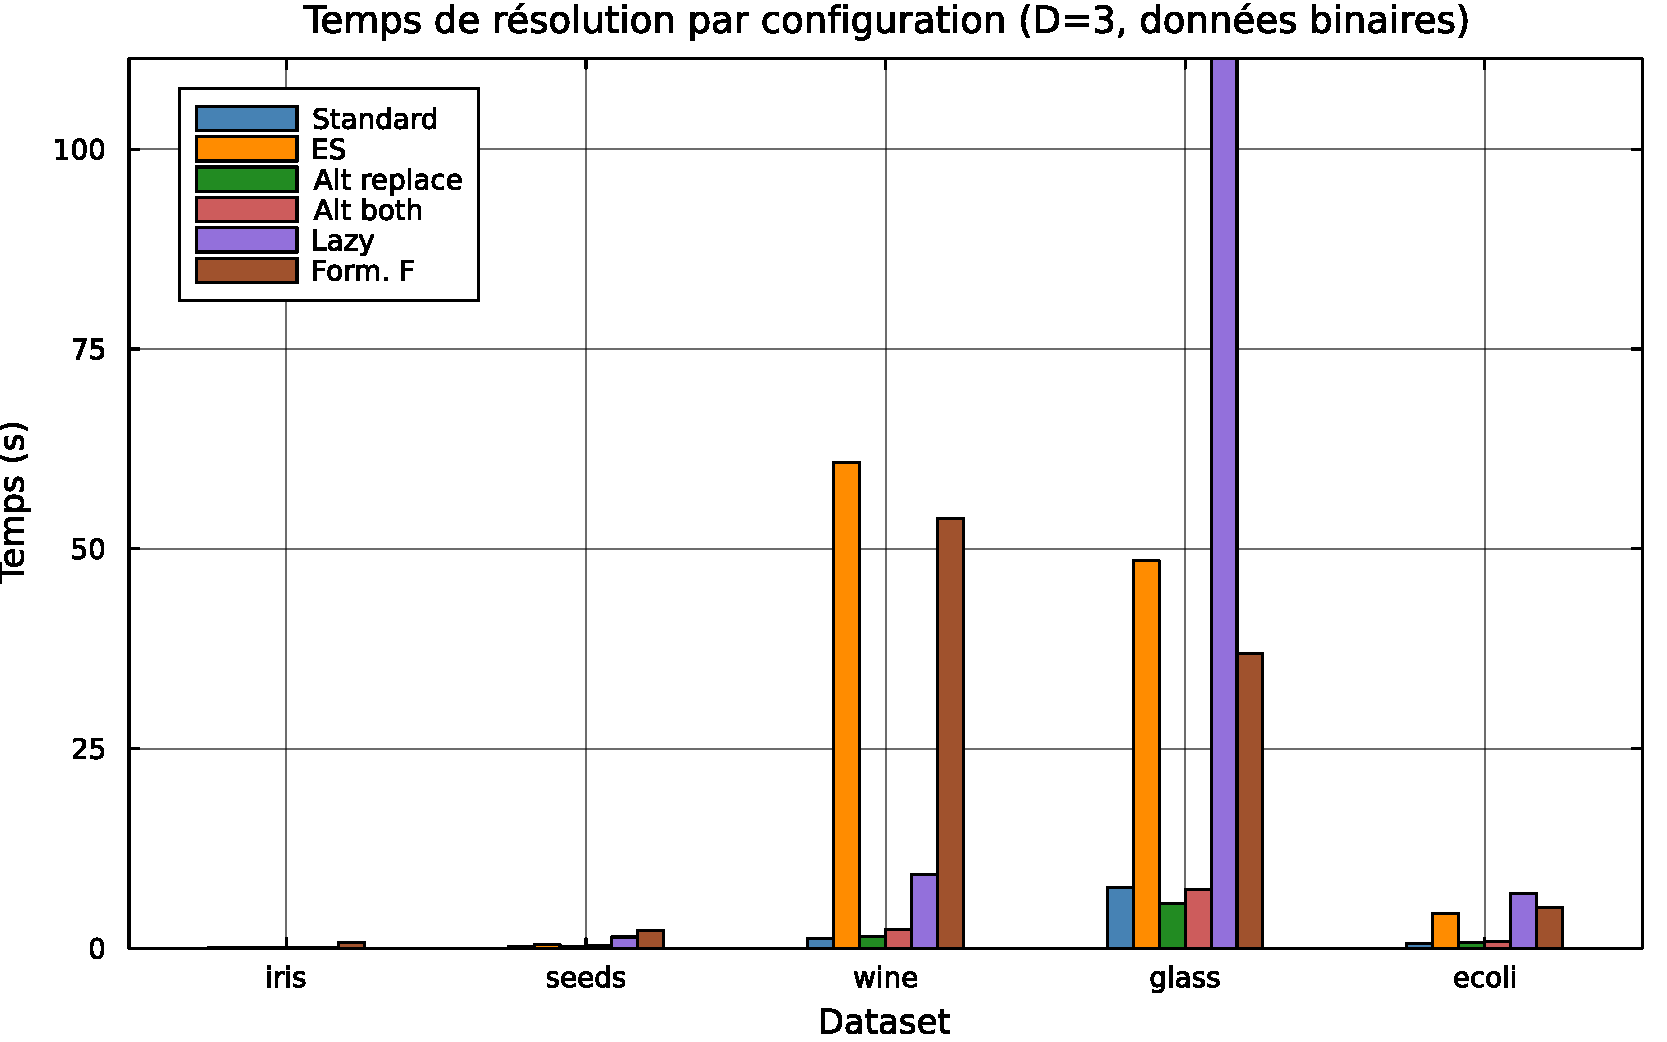
\includegraphics[width=\textwidth]{figures/part4_time_by_config.pdf}
  \caption{Temps par configuration ($D{=}3$).}
\end{subfigure}
\hfill
\begin{subfigure}[t]{0.48\textwidth}
  \centering
  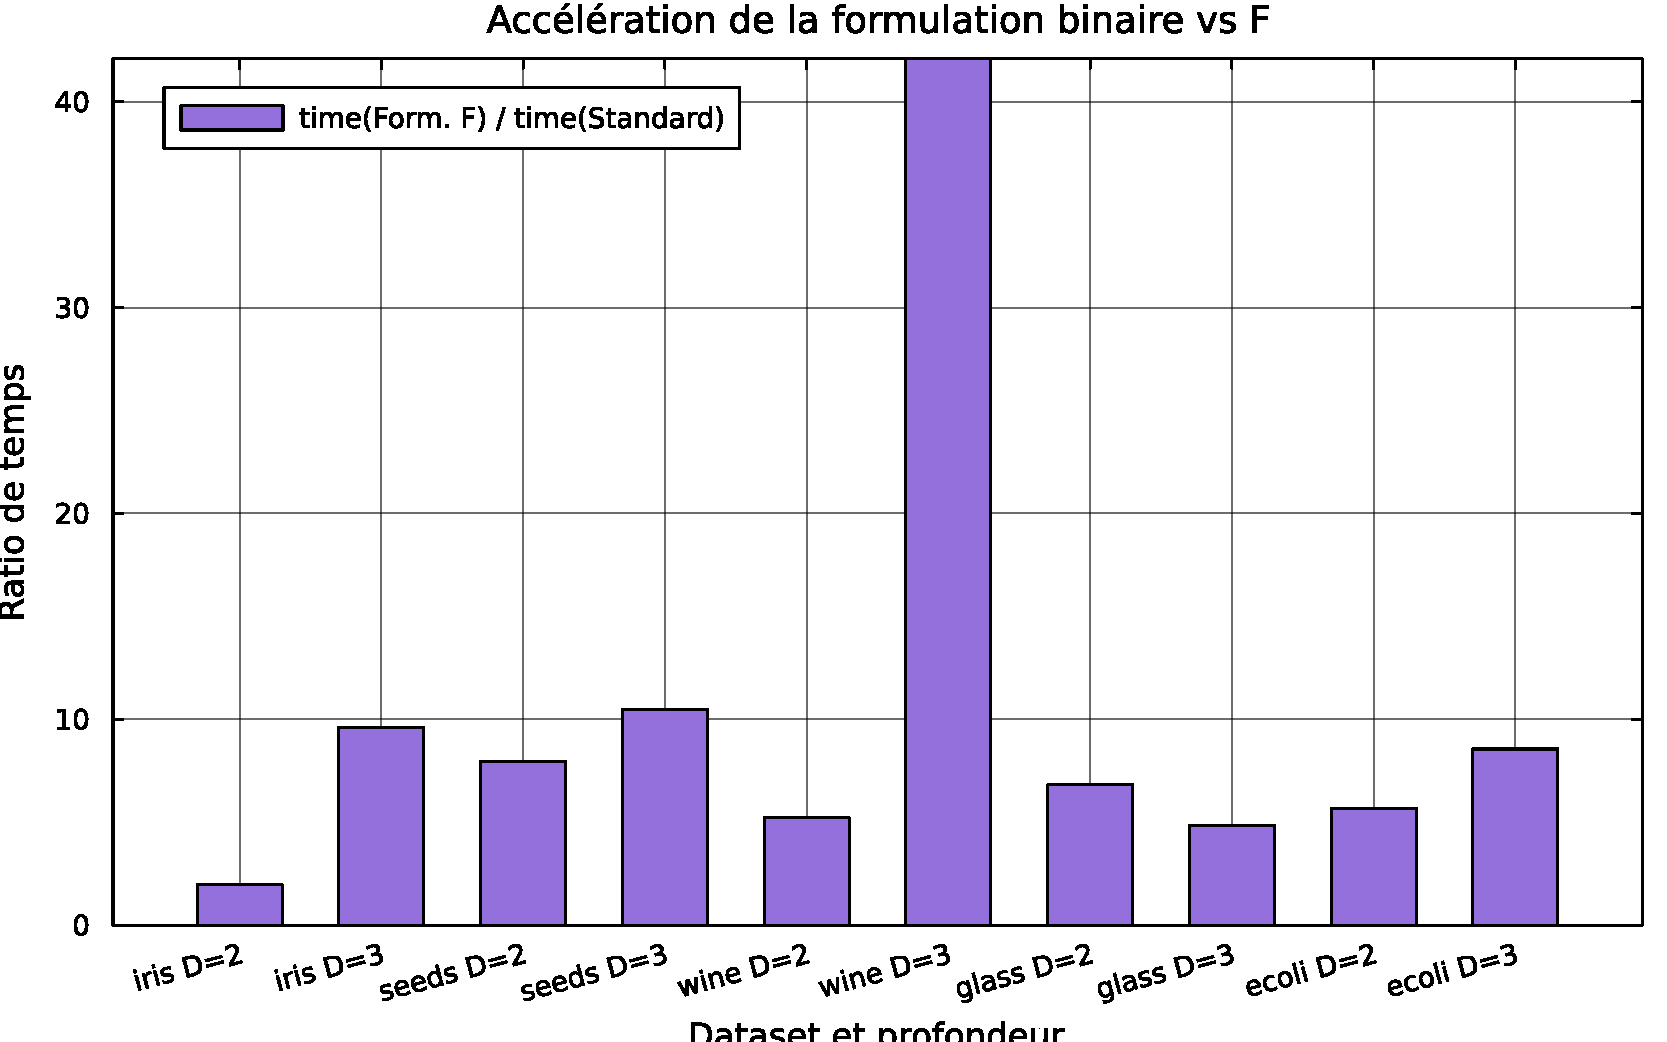
\includegraphics[width=\textwidth]{figures/part4_speedup.pdf}
  \caption{Ratio temps Form.~F / Standard.}
\end{subfigure}
\caption{Performance de la formulation binaire comparée à la formulation~F.}
\label{fig:part4}
\end{figure}

\begin{figure}[H]
\centering
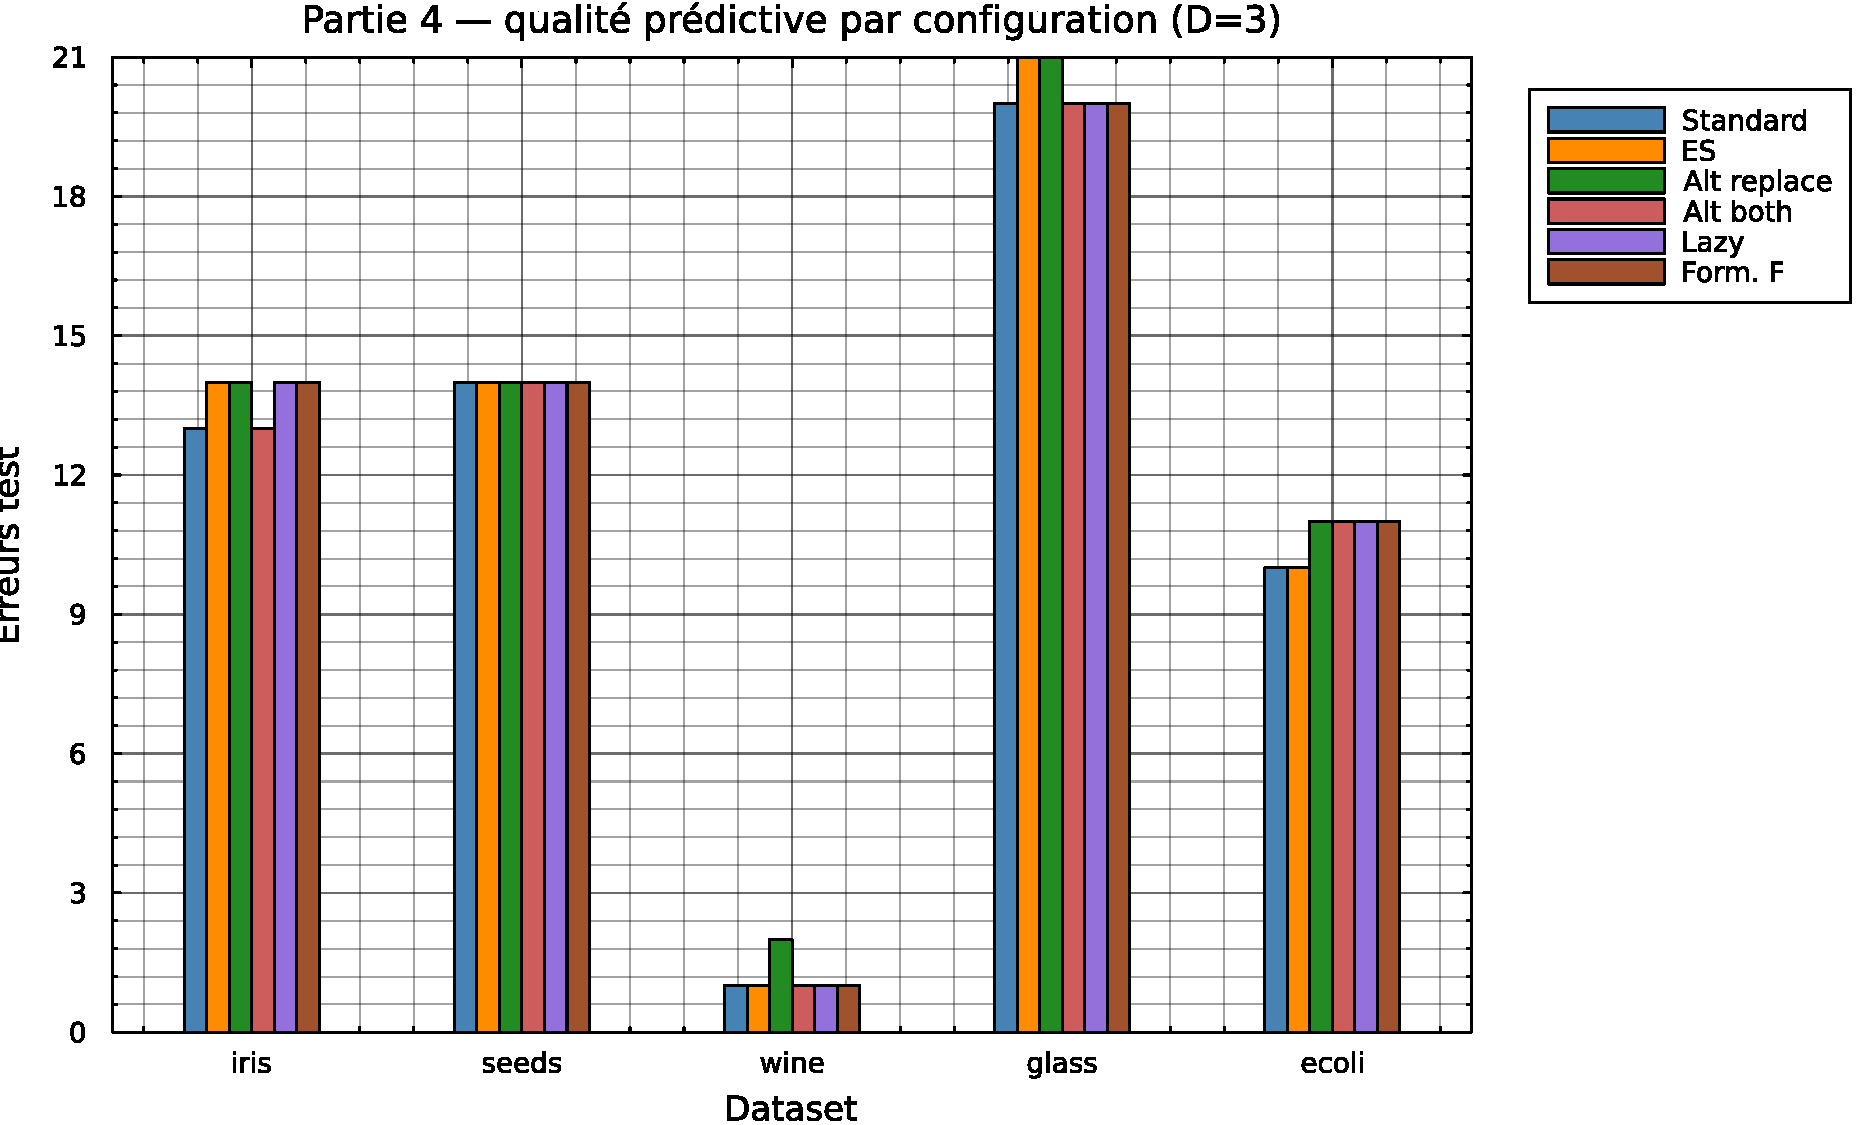
\includegraphics[width=0.72\textwidth]{figures/part4_err_test_by_config_D3.pdf}
\caption{Figure complémentaire Partie~4 : erreurs test par configuration ($D{=}3$).}
\label{fig:part4_enriched}
\end{figure}

\subsection{Analyse}

\begin{resultbox}[Observations clés -- Partie 4]
\begin{itemize}
  \item \textbf{Formulation binaire vs formulation~F.} La variante 5.1 reste en général beaucoup plus rapide que la formulation~F sur les mêmes données binarisées. Exemple marquant : \textbf{wine} à $D{=}3$, $\sim$1{,}3\,s (standard) pour 53\,s (F), avec les mêmes erreurs train/test dans notre tirage.
  \item \textbf{Renforcement ES (5.2).} Ne change pas l'optimum entraînement/test sur la plupart des cas mais peut fortement augmenter le temps (wine $D{=}3$ : $\sim$1{,}3\,s $\to$ $\sim$61\,s) du fait du volume de variables et contraintes supplémentaires.
  \item \textbf{Borne alternative (5.3).} Sur \textbf{iris} $D{=}3$, le standard et \texttt{alt\_both} affichent \textbf{13 erreurs test}, légèrement mieux que ES, \texttt{alt\_replace}, lazy et F (14 dans \texttt{part4\_results.csv}). Sur \textbf{ecoli} $D{=}3$, seuls le standard et ES restent à 10 erreurs test ; \texttt{alt\_replace}, \texttt{alt\_both}, lazy et la formulation~F montent à 11 : de légers écarts selon la formulation malgré un même objectif d'entraînement cible.
  \item \textbf{Lazy callback.} Précision identique au standard sur nos instances, mais coût variable (ex.\ wine $D{=}3$ : 9\,s vs 1{,}3\,s ; glass $D{=}3$ : lazy plus lent que le standard).
  \item \textbf{Impact de la binarisation.} Comme en Partie~1, la discrétisation médiane dégrade fortement le fit (ex.\ iris : 24 erreurs train sur données binaires vs 5 en continu) : c'est une limite du pré-traitement, pas de la seule formulation MIP.
  \item \textbf{Glass} $D{=}3$ : formulation~F reste plus lente que le standard ; ES et lazy peuvent être pénalisants en temps pour un gain de précision nul ou ambigu sur ce jeu.
\end{itemize}
\end{resultbox}


% ══════════════════════════════════════════════════════════════════════════
% ══════════════════════════════════════════════════════════════════════════
\section*{Conclusion}
\addcontentsline{toc}{section}{Conclusion}
% ══════════════════════════════════════════════════════════════════════════
% ══════════════════════════════════════════════════════════════════════════

Ce projet a permis d'explorer quatre directions complémentaires pour enrichir le modèle MIP d'arbres de décision optimaux :

\begin{enumerate}
  \item \textbf{Égalités valides} : les linked sets et opposite box corners permettent de resserrer la relaxation LP et de réduire le nombre de nœuds B\&B, en particulier sur iris (jusqu'à $-40$\,\% de nœuds). L'arrondi des features augmente le nombre d'égalités détectables mais peut dégrader marginalement la qualité de la solution.

  \item \textbf{Équité} : le compromis équité--précision est confirmé sur \texttt{part2\_results.csv}. La contrainte stricte impose un parity gap nul au prix d'une forte dégradation de la précision ; à $D{=}3$, les limites de temps et gaps MIP résiduels doivent être pris en compte pour interpréter les métriques. La tolérance $\varepsilon{=}0{,}15$ reste en pratique un bon compromis lorsque le déséquilibre initial est marqué.

  \item \textbf{Features dérivées} : sélection par gain de Gini améliore nettement \textbf{wine} à $D{=}2$ (précision train/test) et à $D{=}3$ (test $6 \to 4$, temps réduit) ; gain marginal sur \textbf{iris} $D{=}3$ (test $4 \to 3$). Sous limite de temps et fort gap MIP, \textbf{seeds} et \textbf{glass} en $D{=}3$ montrent que l'enrichissement peut dégrader le test.

  \item \textbf{Formulation binaire} : la formulation 5.1 reste typiquement bien plus rapide que la formulation~F sur données binarisées (écarts d'ordre de grandeur sur wine $D{=}3$). ES alourdit souvent la résolution. Les variantes 5.3 modulent parfois légèrement les erreurs test (iris, ecoli) sans effet miracle systématique sur l'échantillon courant.
\end{enumerate}

\paragraph{Jeux de données.} Conformément au sujet, les expériences portent sur les trois jeux fournis (\texttt{iris}, \texttt{seeds}, \texttt{wine}) et sur deux jeux supplémentaires au choix~: \texttt{glass} (classification de types de verre, UCI, 9~features, 6~classes) et \texttt{ecoli} (localisation de protéines, UCI, 7~features, 8~classes), cohérents avec le cadre du projet (classification supervisée, features numériques, arbres de décision optimaux).

\end{document}
